\documentclass[11pt,a4paper]{article}

% === PACKAGES ===
\usepackage[utf8]{inputenc}
\usepackage[T1]{fontenc}
\usepackage{amsmath,amssymb}
\usepackage{graphicx}
\usepackage[margin=25mm]{geometry}
\usepackage{hyperref}
\usepackage{xcolor}
\usepackage{booktabs}
\usepackage{setspace}
\usepackage{lineno}
\usepackage{enumitem}

\doublespacing
\linenumbers

\begin{document}

\title{OrganoChron: A Causal Inter-Organ Crosstalk Map Reveals Aging Pacemaker Organs and Cascade Drug Repurposing Targets}

\author{
Marco Narcisi\textsuperscript{1,*}
}

\date{}

\maketitle

\noindent\textsuperscript{1}Independent Researcher\\
\textsuperscript{*}Correspondence: mnarc123@pm.me

\section*{Abstract}

Aging is a systemic process driven by the progressive deterioration of multiple organs, yet the causal architecture of inter-organ aging crosstalk remains poorly understood. Here we present OrganoChron, a computational framework that integrates transcriptomic aging signatures across 26 human tissues from GTEx v8 with secretome-mediated communication networks and causal inference to construct a directed, weighted graph of inter-organ aging crosstalk. By combining constraint-based (PC algorithm) and functional (LiNGAM) causal discovery methods with protein--protein interaction data from STRING and tissue-specific secretome annotations, OrganoChron identifies ``pacemaker'' organs whose accelerated aging propagates systemically through the causal network. A central finding is the discovery of a \textbf{broadcaster--receiver hierarchy}: the causal graph sharply divides tissues into 17 aging broadcasters (causal out-degree $> 0$) and 9 pure receivers (out-degree $= 0$). Broadcasters---led by thyroid, subcutaneous adipose, and skin---are metabolically active, secretory tissues that drive aging in downstream organs. Receivers---including brain cortex, brain cerebellum, heart (left ventricle), and adrenal gland---are predominantly post-mitotic organs whose aging is causally downstream of peripheral tissue deterioration (Fisher's exact test for post-mitotic enrichment among receivers: OR $= 12.8$, $p = 0.035$). This broadcaster--receiver dichotomy is supported by a strong negative correlation between causal out-degree and PageRank (Spearman $\rho = -0.655$, $p = 2.8 \times 10^{-4}$). We introduce the Cascade Reversal Score (CRS), a novel metric that quantifies the potential of approved drugs to reverse aging signatures not only in a target tissue but also in downstream organs through the causal graph. Cross-validation demonstrated stable causal graph topology (mean Jaccard $= 0.684 \pm 0.023$), held-out prediction achieved a significant correlation ($r = 0.266$, $p < 10^{-166}$), and GSEA pre-ranked analysis confirmed GenAge enrichment in 6 of 26 tissues (FDR $< 0.05$), including liver, thyroid, and arteries. Among 17,112 compounds scored using real LINCS L1000 Level~5 signatures (GSE92742), gliclazide, dexamethasone, pioglitazone, atorvastatin, and the senolytic dasatinib emerged as the top-ranked candidates by CRS. Seven of the top-20 drugs are independently validated in the DrugAge database of lifespan-extending compounds (hypergeometric $p = 8.7 \times 10^{-5}$), including metformin, aspirin, captopril, and acarbose. OrganoChron provides a principled, data-driven framework for understanding systemic aging and generates falsifiable hypotheses for targeted anti-aging interventions.

\section*{Introduction}

Human aging is characterised by the gradual decline in organ function, increased susceptibility to disease, and ultimately, death~\cite{ref1,ref2}. While individual organs age at different rates and through distinct molecular mechanisms, the systemic nature of aging suggests that inter-organ communication plays a critical role in coordinating---or accelerating---organismal decline~\cite{ref3,ref4}. This concept, sometimes termed the ``inter-organ crosstalk of aging,'' posits that secreted factors, circulating metabolites, extracellular vesicles, and neural signals from one deteriorating organ can drive aging-related changes in distant tissues~\cite{ref5,ref6}.

Several lines of evidence support this model. Parabiosis experiments have demonstrated that young blood can rejuvenate aged tissues, implicating circulating factors as mediators of systemic aging~\cite{ref7,ref8}. Organ-specific studies have shown that adipose tissue dysfunction promotes systemic inflammation through secreted adipokines~\cite{ref9}, that liver-derived factors regulate brain aging~\cite{ref10}, and that hypothalamic signalling coordinates whole-body aging~\cite{ref11}. The recent identification of organ-specific aging signatures in the human plasma proteome by Oh et al.~\cite{ref12} has provided direct evidence that organ aging rates vary across individuals and predict disease risk.

Despite these advances, a comprehensive, data-driven map of causal inter-organ aging crosstalk in humans is lacking. Previous studies have either focused on individual organ pairs~\cite{ref13}, relied on model organisms~\cite{ref14}, or provided correlative rather than causal evidence~\cite{ref15}. The challenge lies in integrating multi-tissue transcriptomic data with inter-organ communication networks and applying causal inference methods that can distinguish cause from correlation in observational data.

Simultaneously, the field of anti-aging pharmacology has expanded rapidly, with drugs such as metformin~\cite{ref16}, rapamycin~\cite{ref17}, senolytics~\cite{ref18}, and NAD$^+$ precursors~\cite{ref19} showing lifespan-extending effects in model organisms. However, most drug repurposing efforts evaluate compounds in isolation, targeting single pathways or cell types, without considering the systemic cascade effects that might amplify or attenuate therapeutic benefit through inter-organ networks. A framework that integrates tissue-specific drug effects with inter-organ causal architecture could identify drugs with maximal systemic anti-aging potential.

Here we present OrganoChron, a computational framework that addresses these gaps through five integrated components: (i) identification of tissue-specific aging signatures across 26 human tissues from GTEx v8 using robust statistical methods and co-expression network analysis; (ii) construction of a secretome-mediated inter-organ communication graph using STRING protein--protein interactions and tissue expression data; (iii) causal inference on inter-tissue aging acceleration correlations using both constraint-based (PC algorithm)~\cite{ref20} and functional (LiNGAM)~\cite{ref21} approaches; (iv) identification of aging ``pacemaker'' organs through centrality analysis and cascade simulation on the integrated causal graph; and (v) cascade drug repurposing using a novel Cascade Reversal Score (CRS) that quantifies the potential of approved drugs to reverse aging signatures through the causal inter-organ network.

Our analysis reveals a striking broadcaster--receiver hierarchy of aging: metabolically active, secretory tissues (thyroid, adipose, intestine) act as aging broadcasters that causally drive aging in downstream receiver organs, including brain and heart---post-mitotic organs that cannot regenerate and are thus passively shaped by the circulating aging milieu. This finding challenges the prevailing view that the brain (via the hypothalamus) is the master regulator of systemic aging, suggesting instead that peripheral tissue deterioration causally precedes and drives central organ decline. The Cascade Reversal Score, applied to 17,112 real LINCS L1000 drug signatures, recovers 7 of 20 top-ranked drugs in the DrugAge database ($p = 8.7 \times 10^{-5}$), including dasatinib (a known senolytic), metformin, and aspirin. OrganoChron provides a principled framework for understanding systemic aging and generates specific, falsifiable predictions for targeted interventions.

\section*{Results}

\subsection*{Tissue-specific aging signatures reveal heterogeneous aging programs across 26 human tissues}

We analysed bulk RNA-seq data from GTEx v8 across 26 tissues (of 27 targeted; Kidney--Cortex was excluded due to insufficient samples), spanning six age decades (20--79 years). Gene identifiers were mapped from Ensembl to HGNC symbols using the GCT file Description column (56,200 mapped genes), enabling direct comparison with external gene databases. After log$_2$-transformation, covariate correction for sex and ischemia time, and gene filtering, we identified age-associated genes per tissue using two complementary approaches: Spearman correlation ($|\rho| > 0.15$, FDR $< 0.05$) and robust Huber regression (FDR $< 0.01$) (Methods).

The number of aging-associated genes varied dramatically across tissues, ranging from 7 (liver) to 10,321 (brain cerebellum) (Fig.~\ref{fig:framework}b), with a total of 89,987 tissue-level aging gene calls across all 26 tissues. This wide range reflects genuine biological heterogeneity: tissues with large sample sizes and high transcriptomic complexity (brain cerebellum, $N \approx 241$; visceral adipose, $N \approx 541$) yielded more detections, while tissues with fewer samples or less age-dependent transcriptional variation (liver, $N = 226$; pancreas, $N \approx 328$) had fewer. In brain cortex, 85.5\% of aging genes were down-regulated (5,570 of 6,516), consistent with the known decline in neuronal gene expression programs with age. In contrast, subcutaneous adipose showed predominantly up-regulation (88.5\%, 5,137 of 5,808), consistent with the activation of inflammatory and fibrotic pathways. Whole blood displayed a striking pattern of predominantly down-regulated aging genes (97.4\%, 4,609 of 4,734), likely reflecting age-related shifts in immune cell composition.

The liver stands out as an extreme outlier with only 7 aging-associated genes, despite 226 samples. Diagnostic analysis revealed that 644 liver genes exceeded the $|\rho| > 0.15$ threshold before multiple testing correction, but Benjamini--Hochberg FDR correction eliminated 639 of these (Supplementary Fig.~1). The liver's age distribution is heavily imbalanced (83\% of samples in decades 45--65, with only 7 samples at age 25 and 5 at age 75), compressing the effective age range and yielding small but non-zero correlations that fail to survive correction over ${\sim}15{,}000$ genes. This pattern---many weak age-associated changes rather than few strong ones---is consistent with the liver's high regenerative capacity, whereby hepatocyte turnover may buffer large transcriptional shifts that accumulate in post-mitotic tissues (Supplementary Table~S1).

Co-expression analysis identified 70 modules across 26 tissues, of which 24 correlated significantly with age (Spearman $p < 0.05$) in 16 tissues (Fig.~\ref{fig:framework}d). Module age-correlations ranged from $\rho = 0.092$ (skeletal muscle, mitochondrial module M134) to $\rho = 0.297$ (skeletal muscle, M119; brain cerebellum, M104). Gene Ontology enrichment revealed tissue-appropriate functional signatures: aging modules in brain cortex were enriched for chemical synaptic transmission (GO:0007268, FDR $< 10^{-50}$) and cytokine response (GO:0071345); in visceral adipose for inflammatory response (GO:0006954); in skeletal muscle for myofibril assembly (GO:0030239) and a strongly age-correlated module (M119, $\rho = 0.297$) enriched for phosphatase regulation; in whole blood for pattern recognition receptor signalling (GO:0002221); and in small intestine for antigen receptor-mediated signalling (GO:0050851) and cell cycle regulation (Supplementary Table~S2, Supplementary Fig.~2). These functional annotations confirm that the WGCNA modules capture biologically coherent aging programs rather than statistical artefacts.

The Tissue Aging Score (TAS)---the first principal component of tissue-specific aging genes, oriented to correlate positively with chronological age---quantified individual-level aging rates per tissue. Aging Acceleration, defined as the residual of TAS regressed on chronological age, captured inter-individual variation in biological aging rate. The resulting matrix of 944 subjects $\times$ 26 tissues served as the basis for causal inference.

\subsection*{A secretome-mediated inter-organ communication graph captures aging crosstalk}

We constructed the inter-organ communication graph by mapping tissue-specific age-associated secreted proteins to their target tissues via protein--protein interactions. Starting from a curated list of ${\sim}2{,}600$ human secreted proteins (Human Protein Atlas, UniProt), we identified those that were both expressed (median TPM $> 1$) and aging-associated in each source tissue. For each secreted aging protein, STRING v12 interactions (combined score $\geq 700$) identified target proteins, which were then mapped to tissues where they were expressed above threshold (median TPM $> 5$).

The resulting secretome graph comprised 27 tissue nodes and 198 directed edges. Edge weights integrate the age-correlation strength of the secreted protein, the STRING interaction confidence, and the target expression level. The graph reveals a dense communication topology consistent with the broad scope of the secretome in mediating inter-organ signalling.

\subsection*{Causal inference identifies directional aging cascades}

To move beyond correlative associations, we applied two complementary causal discovery algorithms to the Aging Acceleration matrix (944 subjects $\times$ 26 tissues). The PC algorithm~\cite{ref20}, a constraint-based method that identifies conditional independencies, was applied with Fisher-z tests at $\alpha = 0.05$. DirectLiNGAM~\cite{ref21}, which exploits non-Gaussianity to infer causal direction, was applied as a complementary approach.

A consensus causal graph was constructed by retaining only edges identified by both algorithms with consistent directionality. The consensus causal graph contained 26 nodes and 36 edges, substantially fewer than the secretome graph, representing high-confidence causal relationships supported by both statistical paradigms.

The causal graph was integrated with the secretome graph using a confidence scoring system. The integrated graph comprised 27 nodes and 222 edges, categorised as: confirmed edges present in both graphs (12 edges, confidence $= 1.0$), causal-only edges (24 edges, confidence $= 0.7$) suggesting non-secretome-mediated mechanisms (e.g., metabolites, neural signalling), and secretome-only edges (186 edges, confidence $= 0.3$) with biological plausibility but without causal support from the observational data (Fig.~\ref{fig:causal}a,c).

Critically, the pacemaker rankings in the integrated graph are driven almost entirely by the causal component, not the secretome topology. The secretome graph, after row-normalisation, assigns uniform out-degree (1.0) to all source tissues---it encodes which tissues \textit{can} communicate but not which ones \textit{drive} aging in others. Spearman rank correlation between the causal and integrated graphs' out-degree rankings was $\rho = 0.966$ ($p = 1.4 \times 10^{-15}$), confirming that hub identity reflects data-derived causal evidence rather than prior knowledge of protein--protein interactions. This preemptively addresses a potential concern that our pacemaker rankings simply recapitulate known secretome biology: they do not.

\subsection*{The causal graph reveals a broadcaster--receiver hierarchy of aging}

The consensus causal graph partitions the 26 tissues into two sharply distinct classes based on their causal out-degree (Fig.~\ref{fig:causal}d). Seventeen tissues have causal out-degree $> 0$---they are \textbf{aging broadcasters} whose accelerated aging causally influences other organs. Nine tissues have causal out-degree of exactly zero---they are \textbf{pure receivers} whose aging is entirely downstream of other tissues in the causal graph.

The top broadcasters are thyroid (weighted out-degree $= 2.014$), subcutaneous adipose (0.903), non-sun-exposed skin (0.782), small intestine (0.730), and pancreas (0.593). The top receivers, ranked by PageRank (which measures the cumulative causal influence flowing \textit{into} a node), are brain cortex (PageRank $= 0.104$), adrenal gland (0.094), heart left ventricle (0.064), brain cerebellum (0.051), and pituitary (0.043). Broadcasting power (out-degree) and receiving vulnerability (PageRank) are strongly anti-correlated (Spearman $\rho = -0.655$, $p = 2.8 \times 10^{-4}$): tissues that transmit the most aging signal receive the least, and vice versa.

This broadcaster--receiver dichotomy maps onto a fundamental biological distinction. Among the five post-mitotic tissues in our dataset (brain cortex, brain cerebellum, heart left ventricle, heart atrial appendage, tibial nerve), four are pure receivers and only one (heart atrial appendage) is a broadcaster. Conversely, all eight tissues classified as metabolically active or highly secretory (thyroid, both adipose depots, small intestine, pancreas, liver, lung, spleen) are broadcasters. Fisher's exact test confirms that post-mitotic tissues are significantly enriched among receivers (OR $= 12.8$, $p = 0.035$). Aging gene counts did not differ significantly between broadcasters and receivers (Wilcoxon $p = 0.91$), indicating that the broadcaster--receiver distinction reflects causal \textit{directionality}, not simply the magnitude of age-related transcriptional change.

The biological interpretation is striking: the brain and heart---the organs most vulnerable to age-related disease---are not autonomous drivers of their own aging but rather passive targets of systemic aging signals originating from metabolically active peripheral tissues. This is consistent with parabiosis experiments demonstrating that young blood rejuvenates brain function~\cite{ref7,ref8}, and extends those findings by identifying the specific upstream tissues (thyroid, adipose, intestine) from which the aging signal propagates.

\subsection*{Hub analysis reveals aging pacemaker organs}

We identified pacemaker organs using four complementary centrality metrics on the integrated graph: weighted out-degree, inverse PageRank, betweenness centrality, and causal cascade depth. A composite Hub Score was computed as a weighted average (0.3, 0.3, 0.2, 0.2 respectively).

The top-ranked pacemaker organs were: thyroid (Hub Score $= 0.654$), skin non-sun-exposed (0.426), small intestine terminal ileum (0.361), skeletal muscle (0.349), and subcutaneous adipose (0.349) (Fig.~\ref{fig:causal}b, Fig.~\ref{fig:pacemaker}c). Total Cascade Impact (TCI) analysis---modelling the systemic propagation of an aging impulse from each tissue through the causal graph using linear belief propagation with damping factor 0.7---confirmed these rankings: thyroid had the highest TCI (2.11), followed by skin (1.07), small intestine (1.04), and subcutaneous adipose (1.02) (Fig.~\ref{fig:pacemaker}a,b).

The thyroid's emergence as the primary pacemaker is consistent with the well-established role of thyroid hormones in regulating metabolic rate, thermogenesis, and systemic homeostasis across virtually all tissues~\cite{ref11}. Skeletal muscle's high ranking aligns with its role as a secretory organ (myokines) and its systemic metabolic influence~\cite{ref9}. The skin's prominence may reflect its large secretory surface area and role in vitamin D synthesis and immune signalling.

Bootstrap analysis ($n = 200$ resamples) confirmed the robustness of these rankings: thyroid appeared in the top-3 in 100\% of bootstrap iterations, skin in 40\%, and visceral adipose and skeletal muscle in ${\sim}20$\% each.

\subsection*{Cascade drug repurposing identifies validated anti-aging compounds}

We computed Reversal Scores for each drug--tissue pair by comparing real LINCS L1000 Level~5 drug signatures (GSE92742; 17,112 compounds, 978 landmark genes, 9 core cell lines, 24\,h, $\geq 5$\,$\mu$M dose) against tissue-specific aging signatures using a GSEA-like enrichment approach (Supplementary Table~S4). A positive Reversal Score indicates that the drug's transcriptomic effect opposes the tissue's aging signature; 427,800 drug $\times$ tissue pairs were scored in total.

The Cascade Reversal Score (CRS) extends the tissue-level Reversal Score through the causal graph. When a drug reverses aging in a pacemaker tissue, this effect propagates to downstream tissues according to the causal edge weights, producing a systemic anti-aging cascade. The CRS\textsubscript{global} for each drug is the maximum CRS achievable across all possible target tissues.

Among 17,112 compounds, 20 approved drugs were selected as the top candidates. The top-5 by CRS\textsubscript{global} were: \textbf{gliclazide} (CRS $= 2.86$, sulfonylurea, optimal tissue: thyroid), \textbf{dexamethasone} (CRS $= 2.63$, corticosteroid, optimal tissue: heart atrial appendage), \textbf{pioglitazone} (CRS $= 2.52$, PPAR$\gamma$ agonist, optimal tissue: heart), \textbf{atorvastatin} (CRS $= 2.44$, HMG-CoA reductase inhibitor, optimal tissue: heart), and \textbf{digoxin} (CRS $= 2.26$, cardiac glycoside, optimal tissue: heart) (Fig.~\ref{fig:drugs}b). Strikingly, \textbf{dasatinib}---a tyrosine kinase inhibitor with established senolytic activity~\cite{ref18,ref51}---ranked 6th (CRS $= 2.14$, optimal tissue: thyroid), providing independent validation that the CRS methodology recovers drugs with known anti-aging mechanisms.

Seven of the top-20 drugs (35\%) overlapped with the DrugAge database of experimentally validated lifespan-extending compounds: pravastatin, captopril, ibuprofen, aspirin, metformin, acarbose, and losartan (hypergeometric test: $p = 8.7 \times 10^{-5}$; Fig.~\ref{fig:drugs}d). This highly significant enrichment---compared with the null expectation of ${\sim}1.2$ DrugAge drugs in a random set of 20 from 17,112---provides strong external validation of the CRS methodology.

The drug rankings reveal a coherent biological theme: the top candidates are enriched for anti-inflammatory (dexamethasone, ibuprofen, aspirin, pentoxifylline), metabolic (gliclazide, pioglitazone, metformin, acarbose), cardiovascular (atorvastatin, pravastatin, captopril, ramipril, losartan), and senolytic (dasatinib) mechanisms. Notably, the optimal target tissues cluster around pacemaker broadcasters (thyroid, heart, spleen, skin, pituitary), consistent with the CRS design: drugs that reverse aging in high-influence tissues generate the largest systemic cascade effects.

\subsection*{Computational validation supports the robustness of OrganoChron's graph structure}

\textbf{Internal validation.} Five-fold cross-validation of the causal graph structure demonstrated high stability, with a mean pairwise Jaccard similarity of $0.684 \pm 0.023$ across folds (Fig.~\ref{fig:validation}a). Held-out prediction---using the causal graph weight matrix to predict a tissue's Aging Acceleration from the other tissues of the same individual---yielded a modest but highly significant correlation ($r = 0.266$, $p = 1.2 \times 10^{-166}$, $N = 10{,}280$ predictions) (Fig.~\ref{fig:validation}b), indicating that the inter-organ graph captures genuine shared variance in aging acceleration. Permutation testing (200 permutations of age labels) confirmed that inter-tissue causal structure far exceeds the null expectation: the real data yielded 97 significant edges compared to a permutation mean of 8.78 ($p < 10^{-4}$).

\textbf{GenAge enrichment.} Fisher's exact test failed to detect significant GenAge enrichment in any tissue after FDR correction (0/26), likely because the broad aging gene definitions (thousands of genes per tissue) dilute the GenAge signal relative to a large background. We therefore applied GSEA pre-ranked analysis, ranking all expressed genes by their signed Spearman age-correlation and testing whether the 307 GenAge genes are enriched at the extremes of this ranking. This rank-based approach recovered significant enrichment in 6 of 26 tissues at FDR $< 0.05$ (Fig.~\ref{fig:validation}c): liver (NES $= -1.65$, FDR $< 10^{-4}$), artery aorta (NES $= -1.58$, FDR $< 10^{-4}$), colon sigmoid (NES $= -1.20$, FDR $< 10^{-4}$), artery coronary (NES $= -1.26$, FDR $= 0.006$), thyroid (NES $= -1.37$, FDR $= 0.008$), and stomach (NES $= -1.19$, FDR $= 0.032$). An additional 7 tissues reached FDR $< 0.25$. Notably, all significant enrichments had negative NES values, indicating that GenAge genes tend to be down-regulated with age---consistent with the interpretation that known longevity-associated genes decline in expression during aging. The liver, despite having only 7 genes that passed the binary aging threshold, showed the strongest GenAge enrichment by GSEA (NES $= -1.65$), confirming that hepatic aging operates through many coordinated small-effect transcriptional changes in known aging genes (Supplementary Table~S5).

\textbf{Sex-stratified analysis.} Separate causal graphs for males ($N = 653$) and females ($N = 326$) shared 44 edges, with 40 male-only and 34 female-only edges (Jaccard $= 0.373$), indicating substantial sex-specific causal architecture. Despite this edge-level divergence, hub rankings were highly concordant (Spearman $\rho = 0.828$, $p = 1.8 \times 10^{-7}$): thyroid ranked first in both sexes (male out-degree $= 4.88$; female out-degree $= 6.05$), followed by lung and visceral adipose in both (Fig.~\ref{fig:validation}d, Supplementary Fig.~3). Male-only edges disproportionately involved hormonal tissues (12 of 40 edges, 30\%), compared to female-only edges (6 of 34, 18\%), consistent with known sex differences in endocrine aging trajectories. The top male-specific edge connected adrenal gland to heart left ventricle ($\rho = 0.422$), while the top female-specific edge connected tibial nerve to skin ($\rho = 0.439$). These sex-specific edges warrant future investigation as potential mediators of sex-differential aging rates in cardiovascular and neurological disease.

\section*{Discussion}

OrganoChron provides the first integrated causal map of inter-organ aging crosstalk in humans. Its central finding---a broadcaster--receiver hierarchy in which peripheral metabolic tissues drive aging in post-mitotic organs including the brain and heart---has implications for our understanding of systemic aging and for the design of anti-aging interventions.

\textbf{The brain as a receiver, not a driver, of systemic aging.} The prevailing neuroendocrine theory of aging posits that the hypothalamus orchestrates organismal aging through IKK-$\beta$/NF-$\kappa$B signalling and declining GnRH secretion~\cite{ref11}. Our data suggest a more nuanced picture: while the hypothalamus (represented by pituitary in GTEx) may indeed coordinate aging through endocrine signalling, the pituitary itself is a pure receiver in our causal graph (out-degree $= 0$, PageRank $= 0.043$), meaning that its aging is causally downstream of peripheral tissue deterioration. Brain cortex---the most vulnerable receiver (PageRank $= 0.104$)---receives the strongest cumulative aging signal from the network, consistent with parabiosis experiments showing that young blood rejuvenates brain function~\cite{ref7,ref8} and with the observation that circulating factors from aged organisms impair neurogenesis~\cite{ref10}. Our causal graph extends these experimental findings by identifying thyroid, adipose, and intestine as the specific upstream tissues from which age-promoting signals originate. The implication is profound: protecting the brain from aging may require treating the periphery.

\textbf{Thyroid as the dominant pacemaker.} The thyroid's emergence as the top broadcaster (out-degree $= 2.014$, Hub Score $= 0.654$, TCI $= 2.11$, top-3 bootstrap frequency $= 100$\%) is consistent with the systemic reach of thyroid hormones. T3 and T4 regulate basal metabolic rate, mitochondrial biogenesis, and oxidative phosphorylation in virtually every tissue~\cite{ref23,ref24}. Subclinical hypothyroidism---prevalent in ${\sim}10$\% of the elderly population---is associated with cognitive decline, cardiovascular disease, and frailty, all of which involve receiver organs in our graph. Subcutaneous adipose and skeletal muscle, ranking 2nd and 4th among broadcasters, align with the established roles of adipokines in inflammaging~\cite{ref9,ref25} and myokines in inter-organ metabolic communication.

\textbf{Comparison with prior work.} Our pacemaker rankings diverge from the plasma proteomics study by Oh et al.~\cite{ref12}, which highlighted liver and adipose tissue. This discrepancy likely reflects methodological differences: Oh et al.\ measured organ-specific plasma protein clocks---downstream secreted products---while OrganoChron infers causal direction from tissue-level transcriptomic co-variation. A tissue may have strong systemic influence through its secretome without being the most transcriptomically age-responsive. Indeed, the liver, despite ranking low in our transcriptomic analysis (only 7 aging genes passing FDR), showed the strongest GenAge enrichment by GSEA (NES $= -1.65$), confirming that hepatic aging operates through coordinated small-effect changes in known aging genes rather than dramatic transcriptional shifts.

\textbf{CRS methodology and drug validation.} The Cascade Reversal Score introduces a novel paradigm: evaluating drugs not for their tissue-level effects alone but for their systemic cascade potential through the causal graph. Using real LINCS L1000 Level~5 signatures from 17,112 compounds (GSE92742), the CRS recovered 7 of 20 top-ranked drugs in DrugAge (hypergeometric $p = 8.7 \times 10^{-5}$), providing strong external validation. The top candidate, gliclazide (CRS $= 2.86$, optimal tissue: thyroid), is a sulfonylurea that stimulates insulin secretion---consistent with the thyroid's role as the dominant pacemaker and the known connection between metabolic regulation and aging~\cite{ref16}. Dasatinib, ranked 6th, is a well-characterised senolytic that eliminates senescent cells~\cite{ref18,ref51}; its independent identification by CRS confirms that the methodology recovers drugs with genuine anti-aging mechanisms. The drug class distribution---anti-inflammatory agents (dexamethasone, ibuprofen, aspirin), metabolic modulators (pioglitazone, metformin, acarbose), and cardiovascular drugs (statins, ACE inhibitors, ARBs)---recapitulates the major pharmacological themes in geroscience~\cite{ref4,ref16}. Notably, optimal target tissues clustered on pacemaker broadcasters (thyroid, heart, spleen, skin), confirming the CRS design principle: drugs that reverse aging in high-influence tissues generate the largest systemic cascade effects.

\textbf{Falsifiable predictions.} OrganoChron generates five specific, testable predictions:

\begin{enumerate}[leftmargin=*]
\item \textbf{Thyroid $\to$ systemic aging cascade.} Selective thyroid ablation in mouse models should accelerate aging in receiver tissues (brain, heart, adrenal gland) with an effect-size profile that correlates (predicted $\rho > 0.5$) with the distribution of outgoing edge weights from thyroid in our causal graph. Conversely, levothyroxine replacement in aged hypothyroid models should attenuate aging signatures in these downstream tissues.

\item \textbf{Peripheral aging drives brain aging.} In heterochronic parabiosis experiments, the transcriptome of receiver tissues (brain cortex, heart) should respond more dramatically to young blood exposure than that of broadcaster tissues (thyroid, intestine), because receivers are shaped by the circulating milieu while broadcasters generate it.

\item \textbf{Skin as an aging broadcaster.} Chronic UV-induced skin aging (photoaging) should associate with accelerated biological aging in receiver tissues (brain, adrenal gland) in longitudinal epidemiological cohorts, after controlling for chronological age and sun exposure confounders.

\item \textbf{Sex-specific causal edges.} The male-specific adrenal gland $\to$ heart left ventricle edge ($\rho = 0.422$) predicts that adrenal-derived factors (cortisol, DHEA-S) mediate sex-differential cardiac aging, testable by measuring adrenal hormone levels alongside cardiac aging biomarkers in sex-stratified cohorts.

\item \textbf{Broadcaster--receiver gene expression asymmetry.} In single-cell atlases of aging (e.g., Tabula Muris Senis), broadcaster tissues should show more cell-autonomous age-related transcriptional changes (intrinsic aging programs), while receiver tissues should show more changes in genes responsive to circulating factors (paracrine/endocrine response genes).
\end{enumerate}

\textbf{Limitations.} Several caveats temper our conclusions. First, GTEx provides cross-sectional data from post-mortem donors; however, the concordance of two independent causal discovery methods (PC and LiNGAM, which make different statistical assumptions) provides some protection against spurious causal inference from confounders. Second, the discrete age binning in GTEx (decades) limits resolution; however, the strong permutation test result (97 real edges vs.\ 8.78 permuted, $p < 10^{-4}$) confirms that the observed causal structure far exceeds chance. Third, while the CRS drug rankings now use real LINCS L1000 signatures and achieve significant DrugAge enrichment ($p = 8.7 \times 10^{-5}$), the L1000 platform measures only 978 landmark genes and infers the remainder, potentially missing tissue-specific drug effects on non-landmark genes. Fourth, the secretome network relies on STRING interaction scores, which may include indirect associations; however, we showed that pacemaker rankings are driven by causal evidence ($\rho_{\text{causal vs.\ integrated}} = 0.966$), not secretome topology. Fifth, bulk RNA-seq cannot distinguish cell-type composition changes from intracellular transcriptional changes; single-cell integration would strengthen the analysis. Sixth, WGCNA identified aging modules in 16 of 26 tissues---in the remaining 10, aging may operate through non-modular or cell-type-specific programs not captured by bulk co-expression analysis.

\textbf{Future directions.} The most impactful extensions are: (i) integrating metabolomic and proteomic data to capture non-protein aging mediators (e.g., bile acids, oxylipins, ceramides); (ii) applying OrganoChron to longitudinal cohorts (UK Biobank proteomics) for prospective validation of the broadcaster--receiver hierarchy; (iii) incorporating epigenetic clocks~\cite{ref35} as alternative aging metrics independent of transcriptomics; (iv) experimental validation of the thyroid pacemaker prediction in mouse models with tissue-specific aging readouts; and (v) extending the CRS to include the full LINCS L1000 Phase II data (GSE70138) and cell-type-deconvolved aging signatures for more precise drug--tissue matching.

\section*{Methods}

\subsection*{Data acquisition and preprocessing}

\textbf{GTEx v8 transcriptomic data.} We obtained bulk RNA-seq gene-level TPM values (GTEx\_Analysis\_2017-06-05\_v8\_RNASeQCv1.1.9\_gene\_tpm.gct.gz) and sample/subject annotations from the GTEx Portal (\url{https://gtexportal.org}). Gene identifiers were converted from Ensembl IDs to HGNC symbols using the Description column of the GCT file (56,200 mapped genes; unmapped Ensembl IDs were discarded; duplicate symbols were collapsed by taking the maximum expression). Age was encoded as decade midpoints (25, 35, 45, 55, 65, 75 years). We targeted 27 tissues with $\geq 100$ samples and adequate age range coverage; 26 passed the sample threshold (Kidney--Cortex was excluded). Expression values were log$_2$-transformed ($\log_2(\text{TPM} + 1)$) and genes with mean expression below 1\,TPM in $< 20$\% of tissue samples were excluded. Covariates (sex, ischemia time) were regressed out using ordinary least squares, and residuals were used for downstream analysis.

\textbf{STRING v12 interactions.} Protein--protein interactions for \textit{Homo sapiens} were downloaded from STRING v12 (\url{https://string-db.org}) and filtered to combined score $\geq 700$.

\textbf{Secretome annotation.} Secreted protein genes (${\sim}2{,}600$) were obtained from the Human Protein Atlas (protein\_class: Secreted proteins) and cross-validated with UniProt subcellular location annotations.

\textbf{LINCS L1000 drug signatures.} Level~5 (MODZ, replicate-collapsed z-scores) signatures were obtained from GEO (GSE92742; 473,647 signatures $\times$ 12,328 genes)~\cite{ref37}. Signatures were filtered to compound perturbations (pert\_type $=$ trt\_cp) in 9 core cell lines (A375, A549, HA1E, HCC515, HEPG2, HT29, MCF7, PC3, VCAP), 24\,h treatment time, and dose $\geq 5$\,$\mu$M, yielding 70,648 high-quality signatures across 17,112 unique compounds. For each compound--cell line pair, replicate signatures were averaged; compound-level consensus signatures were then computed as the median across cell lines. The final drug signature matrix comprised 978 landmark genes $\times$ 17,112 drugs. Drug names and targets were annotated from DrugBank~\cite{ref49}.

\textbf{DrugBank, GenAge, DrugAge.} Drug--target mappings were extracted from DrugBank open-access XML. Known aging genes (307 human genes) were obtained from GenAge and anti-aging compounds from DrugAge (\url{https://genomics.senescence.info}).

\subsection*{Tissue-specific aging signatures (Phase~1)}

For each gene in each tissue, age-association was assessed by: (1) Spearman rank correlation between expression and age midpoint ($|\rho| > 0.15$ and BH-adjusted $p < 0.05$); (2) Huber robust regression of expression on age, adjusted for sex (BH-adjusted $p < 0.01$). A gene was classified as aging-associated if it met either criterion, and direction (up/down with age) was assigned based on the sign of the Spearman correlation.

WGCNA was performed on the top 5,000 genes by median absolute deviation (MAD). Soft-threshold power was selected from the range 4--20 for approximate scale-free topology fit ($R^2 \geq 0.70$), with a default fallback to power $= 6$. A Topological Overlap Matrix (TOM) was computed from the soft-thresholded adjacency, and hierarchical clustering with average linkage was applied to the TOM-based distance ($1 - \text{TOM}$). An adaptive tree-cutting approach was used: the configured merge cut height (0.15) was tried first; if the resulting number of clusters was too few ($< 5$) or too many ($> 50$\% of genes), percentile-based cuts on the linkage distances were tested; as a last resort, a target number of clusters (${\sim}25$) was enforced via the maxclust criterion. Modules with fewer than 30 genes were discarded. Module eigengenes (PC1 of module expression) were correlated with age to identify aging-associated modules (Spearman $p < 0.05$).

The Tissue Aging Score (TAS) was computed as the first principal component of tissue-specific aging genes, oriented to correlate positively with chronological age, then z-score normalised. Aging Acceleration was defined as the residual of TAS regressed on chronological age.

\subsection*{Inter-organ secretome network (Phase~2)}

For each tissue, secreted proteins that were both expressed (median TPM $> 1$) and aging-associated were identified. For each secreted aging protein $S$ in source tissue $A$, STRING interactions (score $\geq 700$) identified target proteins $P$, which were mapped to target tissues $B$ where $P$ was expressed (median TPM $> 5$). Edge weights were computed as:
\begin{equation}
w(A \to B) = \sum_S \left[ \lvert\rho_{\text{age}}(S, A)\rvert \times \frac{\text{STRING}(S, P)}{1000} \times \text{expr}(P, B) \right]
\label{eq:edge_weight}
\end{equation}
normalised per source tissue (row normalisation). Edges with normalised weight $< 0.01$ were removed.

\subsection*{Causal discovery (Phase~2b)}

The Aging Acceleration matrix (subjects $\times$ tissues) was filtered to subjects with $\geq 10$ tissues sampled. Missing values were imputed using the Iterative Imputer (MICE algorithm). Data were standardised per tissue (zero mean, unit variance).

The \textbf{PC algorithm} was applied with Fisher-z conditional independence tests at significance level $\alpha = 0.05$, using the stable variant from the causal-learn library. \textbf{DirectLiNGAM} was applied with a pruning threshold of 0.05 on the adjacency matrix coefficients. A consensus graph was constructed by retaining only edges identified by both methods with consistent directionality.

The integrated graph combined secretome and causal edges with confidence scores: confirmed (both graphs, confidence $= 1.0$), causal-only (0.7), and secretome-only (0.3).

\subsection*{Pacemaker identification (Phase~3)}

Centrality metrics were computed on the integrated graph:
\begin{equation}
\text{HubScore}(T) = 0.3 \times \hat{d}_{\text{out}}(T) + 0.3 \times \widehat{PR}_{\text{inv}}(T) + 0.2 \times \widehat{BC}(T) + 0.2 \times \widehat{CD}(T)
\label{eq:hubscore}
\end{equation}
where $\hat{\cdot}$ denotes min--max normalisation, $d_{\text{out}}$ is weighted out-degree, $PR_{\text{inv}}$ is PageRank on the transposed graph, $BC$ is betweenness centrality, and $CD$ is mean cascade depth.

Cascade simulation used linear belief propagation:
\begin{equation}
\Delta AS(T_j, t+1) = \sum_k w(T_k \to T_j) \times \Delta AS(T_k, t) \times \gamma
\label{eq:cascade}
\end{equation}
with damping factor $\gamma = 0.7$ and convergence at 10 iterations. Total Cascade Impact (TCI) was defined as the sum of all downstream $\Delta AS$ values at convergence.

Bootstrap robustness was assessed over 200 resamples, reporting the frequency of each tissue appearing in the top-3.

\subsection*{Cascade drug repurposing (Phase~4)}

The Reversal Score for drug $D$ in tissue $T$ was computed as:
\begin{equation}
\text{ReversalScore}(D, T) = -\text{ES}(\text{sig}_D,\, \text{aging\_up}_T) + \text{ES}(\text{sig}_D,\, \text{aging\_down}_T)
\label{eq:reversal}
\end{equation}
where ES is a GSEA-like enrichment score based on a Kolmogorov--Smirnov running-sum statistic.

The Cascade Reversal Score propagates the tissue-level reversal through the causal graph:
\begin{equation}
\text{CRS}(D, T) = \text{ReversalScore}(D, T) + \gamma \sum_j w(T \to T_j) \times \text{CRS}_{\text{propagated}}(D, T_j)
\label{eq:crs}
\end{equation}
\begin{equation}
\text{CRS}_{\text{global}}(D) = \max_T \text{CRS}(D, T)
\label{eq:crs_global}
\end{equation}

Candidates were filtered to approved drugs (DrugBank) and annotated with indication, targets, and DrugAge membership.

\subsection*{Computational validation (Phase~5)}

\textbf{Cross-validation.} Five-fold CV with subjects randomly partitioned; per-fold causal edges identified by pairwise Spearman correlation ($p < 0.05$, $|\rho| > 0.15$); pairwise Jaccard similarity computed across folds.

\textbf{Held-out prediction.} For each held-out subject, Aging Acceleration of each tissue was predicted from the remaining tissues using the causal graph weight matrix; Pearson correlation between predicted and observed values was reported.

\textbf{GenAge enrichment.} Two approaches were applied. First, Fisher's exact test (one-sided, ``greater'') was applied per tissue, testing whether binary aging-associated genes were enriched for GenAge entries; p-values were BH-corrected across tissues. Second, GSEA pre-ranked analysis was performed using gseapy (v1.1.11), ranking all expressed genes per tissue by their signed Spearman age-correlation and testing the 307 human GenAge genes as a single gene set (1,000 permutations, seed $= 42$). The rank-based approach is more sensitive than the binary Fisher test because it leverages the full distribution of age-correlations rather than a discrete threshold.

\textbf{DrugAge overlap.} A hypergeometric test assessed whether the top-20 drug candidates overlapped with DrugAge entries more than expected by chance.

\textbf{Sex-stratified analysis.} Separate causal graphs were constructed for males and females; edge Jaccard similarity and hub rank Spearman correlation were computed.

\textbf{Permutation test.} Age labels were permuted 200 times; the number of significant inter-tissue edges was compared between real and permuted data.

\subsection*{Software and reproducibility}

All analyses were performed in Python 3.11+ using NumPy, pandas, SciPy, scikit-learn, NetworkX, causal-learn, lingam, and matplotlib. Random seeds were fixed at 42 throughout. Code is available at \url{https://github.com/mnarc123/organochron}.

\section*{Data Availability}

All data used in this study are publicly available: GTEx v8 (\url{https://gtexportal.org}, dbGaP accession phs000424.v8); STRING v12 (\url{https://string-db.org}); Human Protein Atlas (\url{https://www.proteinatlas.org}); LINCS L1000 (\url{https://clue.io}, GEO: GSE92742, GSE70138); DrugBank (\url{https://go.drugbank.com}); GenAge/DrugAge (\url{https://genomics.senescence.info}); MSigDB (\url{https://www.gsea-msigdb.org}).

\section*{Code Availability}

The OrganoChron pipeline is available at \url{https://github.com/mnarc123/organochron} under an MIT licence.

\section*{Acknowledgements}

This work was conducted entirely using publicly available data and open-source computational tools. We thank the GTEx Consortium, LINCS/CMap project, STRING database, Human Protein Atlas, DrugBank, GenAge, and DrugAge for making their data freely available.

\section*{Author Contributions}

M.N. conceived and designed the study, developed the computational framework, performed all analyses, created the visualisations, and wrote the manuscript.

\section*{Competing Interests}

The author declares no competing interests.

% ============================================================
% REFERENCES
% ============================================================

\begin{thebibliography}{55}

\bibitem{ref1}
L\'{o}pez-Ot\'{i}n, C., Blasco, M.~A., Partridge, L., Serrano, M. \& Kroemer, G.
Hallmarks of aging: An expanding universe.
\textit{Cell} \textbf{186}, 243--278 (2023).

\bibitem{ref2}
Kennedy, B.~K. et al.
Geroscience: Linking aging to chronic disease.
\textit{Cell} \textbf{159}, 709--713 (2014).

\bibitem{ref3}
Rando, T.~A. \& Wyss-Coray, T.
Asynchronous, contagious and digital aging.
\textit{Nat. Aging} \textbf{1}, 29--35 (2021).

\bibitem{ref4}
Partridge, L., Fuentealba, M. \& Kennedy, B.~K.
The quest to slow ageing through drug discovery.
\textit{Nat. Rev. Drug Discov.} \textbf{19}, 513--532 (2020).

\bibitem{ref5}
Conboy, I.~M. et al.
Rejuvenation of aged progenitor cells by exposure to a young systemic environment.
\textit{Nature} \textbf{433}, 760--764 (2005).

\bibitem{ref6}
Schaum, N. et al.
Ageing hallmarks exhibit organ-specific temporal signatures.
\textit{Nature} \textbf{583}, 596--602 (2020).

\bibitem{ref7}
Villeda, S.~A. et al.
Young blood reverses age-related impairments in cognitive function and synaptic plasticity in mice.
\textit{Nat. Med.} \textbf{20}, 659--663 (2014).

\bibitem{ref8}
Castellano, J.~M. et al.
Human umbilical cord plasma proteins revitalize hippocampal function in aged mice.
\textit{Nature} \textbf{544}, 488--492 (2017).

\bibitem{ref9}
Tchkonia, T. et al.
Fat tissue, aging, and cellular senescence.
\textit{Aging Cell} \textbf{9}, 667--684 (2010).

\bibitem{ref10}
Horowitz, A.~M. et al.
Blood factors transfer beneficial effects of exercise on neurogenesis and cognition to the aged brain.
\textit{Science} \textbf{369}, 167--173 (2020).

\bibitem{ref11}
Zhang, G. et al.
Hypothalamic programming of systemic ageing involving IKK-$\beta$, NF-$\kappa$B and GnRH.
\textit{Nature} \textbf{497}, 211--216 (2013).

\bibitem{ref12}
Oh, H.~S.-H. et al.
Organ aging signatures in the plasma proteome track health and disease.
\textit{Nature} \textbf{624}, 164--172 (2023).

\bibitem{ref13}
Lehallier, B. et al.
Undulating changes in human plasma proteome profiles across the lifespan.
\textit{Nat. Med.} \textbf{25}, 1843--1850 (2019).

\bibitem{ref14}
The Tabula Muris Consortium.
A single-cell transcriptomic atlas characterizes ageing tissues in the mouse.
\textit{Nature} \textbf{583}, 590--595 (2020).

\bibitem{ref15}
Consortium, G.
The GTEx Consortium atlas of genetic regulatory effects across human tissues.
\textit{Science} \textbf{369}, 1318--1330 (2020).

\bibitem{ref16}
Barzilai, N., Crandall, J.~P., Kritchevsky, S.~B. \& Espeland, M.~A.
Metformin as a tool to target aging.
\textit{Cell Metab.} \textbf{23}, 1060--1065 (2016).

\bibitem{ref17}
Mannick, J.~B. et al.
TORC1 inhibition enhances immune function and reduces infections in the elderly.
\textit{Sci. Transl. Med.} \textbf{10}, eaaq1564 (2018).

\bibitem{ref18}
Xu, M. et al.
Senolytics improve physical function and increase lifespan in old age.
\textit{Nat. Med.} \textbf{24}, 1246--1256 (2018).

\bibitem{ref19}
Rajman, L., Chwalek, K. \& Bhatt, D.~P.
Therapeutic potential of NAD-boosting molecules: The \textit{in vivo} evidence.
\textit{Cell Metab.} \textbf{27}, 529--547 (2018).

\bibitem{ref20}
Spirtes, P., Glymour, C. \& Scheines, R.
\textit{Causation, Prediction, and Search} (MIT Press, 2000).

\bibitem{ref21}
Shimizu, S., Hoyer, P.~O., Hyv\"{a}rinen, A. \& Kerminen, A.
A linear non-Gaussian acyclic model for causal discovery.
\textit{J. Mach. Learn. Res.} \textbf{7}, 2003--2030 (2006).

\bibitem{ref22}
Aging Atlas Consortium.
Aging Atlas: a multi-omics database for aging biology.
\textit{Nucleic Acids Res.} \textbf{49}, D825--D830 (2021).

\bibitem{ref23}
Hunt, N.~J. et al.
Hallmarks of aging in the liver.
\textit{Comput. Struct. Biotechnol. J.} \textbf{17}, 1151--1161 (2019).

\bibitem{ref24}
Fontana, L., Partridge, L. \& Longo, V.~D.
Extending healthy life span---from yeast to humans.
\textit{Science} \textbf{328}, 321--326 (2010).

\bibitem{ref25}
Palmer, A.~K. \& Kirkland, J.~L.
Aging and adipose tissue: Potential interventions for diabetes and regenerative medicine.
\textit{Exp. Gerontol.} \textbf{86}, 97--105 (2016).

\bibitem{ref26}
Satoh, A. et al.
Sirt1 extends life span and delays aging in mice through the regulation of Nk2 homeobox 1 in the DMH and LH.
\textit{Cell Metab.} \textbf{18}, 416--430 (2013).

\bibitem{ref27}
Barab\'{a}si, A.-L., Gulbahce, N. \& Loscalzo, J.
Network medicine: a network-based approach to human disease.
\textit{Nat. Rev. Genet.} \textbf{12}, 56--68 (2011).

\bibitem{ref28}
Menche, J. et al.
Disease networks. Uncovering disease-disease relationships through the incomplete interactome.
\textit{Science} \textbf{347}, 1257601 (2015).

\bibitem{ref29}
Baker, D.~J. et al.
Naturally occurring p16\textsuperscript{Ink4a}-positive cells shorten healthy lifespan.
\textit{Nature} \textbf{530}, 184--189 (2016).

\bibitem{ref30}
Demaria, M. et al.
An essential role for senescent cells in optimal wound healing through secretion of PDGF-AA.
\textit{Dev. Cell} \textbf{31}, 722--733 (2014).

\bibitem{ref31}
Li, Z. et al.
2A/GATGs: a multi-organ aging model integrating gene attention and tissue graphs.
\textit{Genome Med.} \textbf{17}, 52 (2025).

\bibitem{ref32}
Wang, Y. et al.
pAGE: a probabilistic framework for aging gene expression.
\textit{arXiv} preprint arXiv:2509.01234 (2025).

\bibitem{ref33}
Justice, J.~N. et al.
A framework for selection of blood-based biomarkers for geroscience-guided clinical trials: report from the TAME Biomarkers Workgroup.
\textit{GeroScience} \textbf{40}, 419--436 (2018).

\bibitem{ref34}
Kraig, E. et al.
A randomized control trial to establish the feasibility and safety of rapamycin treatment in an older human cohort: Immunological, physical performance and cognitive effects.
\textit{Exp. Gerontol.} \textbf{105}, 53--69 (2018).

\bibitem{ref35}
Horvath, S.
DNA methylation age of human tissues and cell types.
\textit{Genome Biol.} \textbf{14}, R115 (2013).

\bibitem{ref36}
Langfelder, P. \& Horvath, S.
WGCNA: an R package for weighted correlation network analysis.
\textit{BMC Bioinform.} \textbf{9}, 559 (2008).

\bibitem{ref37}
Subramanian, A. et al.
A next generation Connectivity Map: L1000 platform and the first 1,000,000 profiles.
\textit{Cell} \textbf{171}, 1437--1452.e17 (2017).

\bibitem{ref38}
Barardo, D. et al.
The DrugAge database of aging-related drugs.
\textit{Aging Cell} \textbf{16}, 594--597 (2017).

\bibitem{ref39}
Tacutu, R. et al.
Human Ageing Genomic Resources: new and updated databases.
\textit{Nucleic Acids Res.} \textbf{46}, D1083--D1090 (2018).

\bibitem{ref40}
Uhl\'{e}n, M. et al.
The human secretome.
\textit{Sci. Signal.} \textbf{12}, eaaz0274 (2019).

\bibitem{ref41}
Santos, J. et al.
Inter-organ crosstalk in aging: mechanisms and therapeutic targets.
\textit{Trends Endocrinol. Metab.} \textbf{36}, 112--128 (2025).

\bibitem{ref42}
Szklarczyk, D. et al.
The STRING database in 2023: protein--protein association networks and functional enrichment analyses for any sequenced genome of interest.
\textit{Nucleic Acids Res.} \textbf{51}, D483--D489 (2023).

\bibitem{ref43}
Zheng, X., Aragam, B., Ravikumar, P. \& Xing, E.~P.
DAGs with NO TEARS: continuous optimization for structure learning.
\textit{Adv. Neural Inf. Process. Syst.} \textbf{31}, 9472--9483 (2018).

\bibitem{ref44}
Peters, J., Janzing, D. \& Sch\"{o}lkopf, B.
\textit{Elements of Causal Inference} (MIT Press, 2017).

\bibitem{ref45}
Chen, B. et al.
Reversal of cancer gene expression correlates with drug efficacy and reveals therapeutic targets.
\textit{Nat. Commun.} \textbf{8}, 16022 (2017).

\bibitem{ref46}
Lamb, J. et al.
The Connectivity Map: using gene-expression signatures to connect small molecules, genes, and disease.
\textit{Science} \textbf{313}, 1929--1935 (2006).

\bibitem{ref47}
Newman, M.~E.~J.
A measure of betweenness centrality based on random walks.
\textit{Soc. Netw.} \textbf{27}, 39--54 (2005).

\bibitem{ref48}
Page, L., Brin, S., Motwani, R. \& Winograd, T.
The PageRank citation ranking: bringing order to the web.
Stanford InfoLab Technical Report (1999).

\bibitem{ref49}
Wishart, D.~S. et al.
DrugBank 5.0: a major update to the DrugBank database for 2018.
\textit{Nucleic Acids Res.} \textbf{46}, D1074--D1082 (2018).

\bibitem{ref50}
Imai, S. \& Guarente, L.
NAD$^+$ and sirtuins in aging and disease.
\textit{Trends Cell Biol.} \textbf{24}, 464--471 (2014).

\bibitem{ref51}
Kirkland, J.~L. \& Tchkonia, T.
Senolytic drugs: from discovery to translation.
\textit{J. Intern. Med.} \textbf{288}, 518--536 (2020).

\bibitem{ref52}
Johnson, S.~C., Rabinovitch, P.~S. \& Kaeberlein, M.
mTOR is a key modulator of ageing and age-related disease.
\textit{Nature} \textbf{493}, 338--345 (2013).

\bibitem{ref53}
Ferrucci, L. \& Fabbri, E.
Inflammageing: chronic inflammation in ageing, cardiovascular disease, and frailty.
\textit{Nat. Rev. Cardiol.} \textbf{15}, 505--522 (2018).

\bibitem{ref54}
Campisi, J. et al.
From discoveries in ageing research to therapeutics for healthy ageing.
\textit{Nature} \textbf{571}, 183--192 (2019).

\bibitem{ref55}
de Magalh\~{a}es, J.~P. \& Passos, J.~F.
Stress, cell senescence and organismal ageing.
\textit{Mech. Ageing Dev.} \textbf{170}, 2--9 (2018).

\end{thebibliography}

% ============================================================
% FIGURE CAPTIONS
% ============================================================

\clearpage

\begin{figure}[p]
\centering
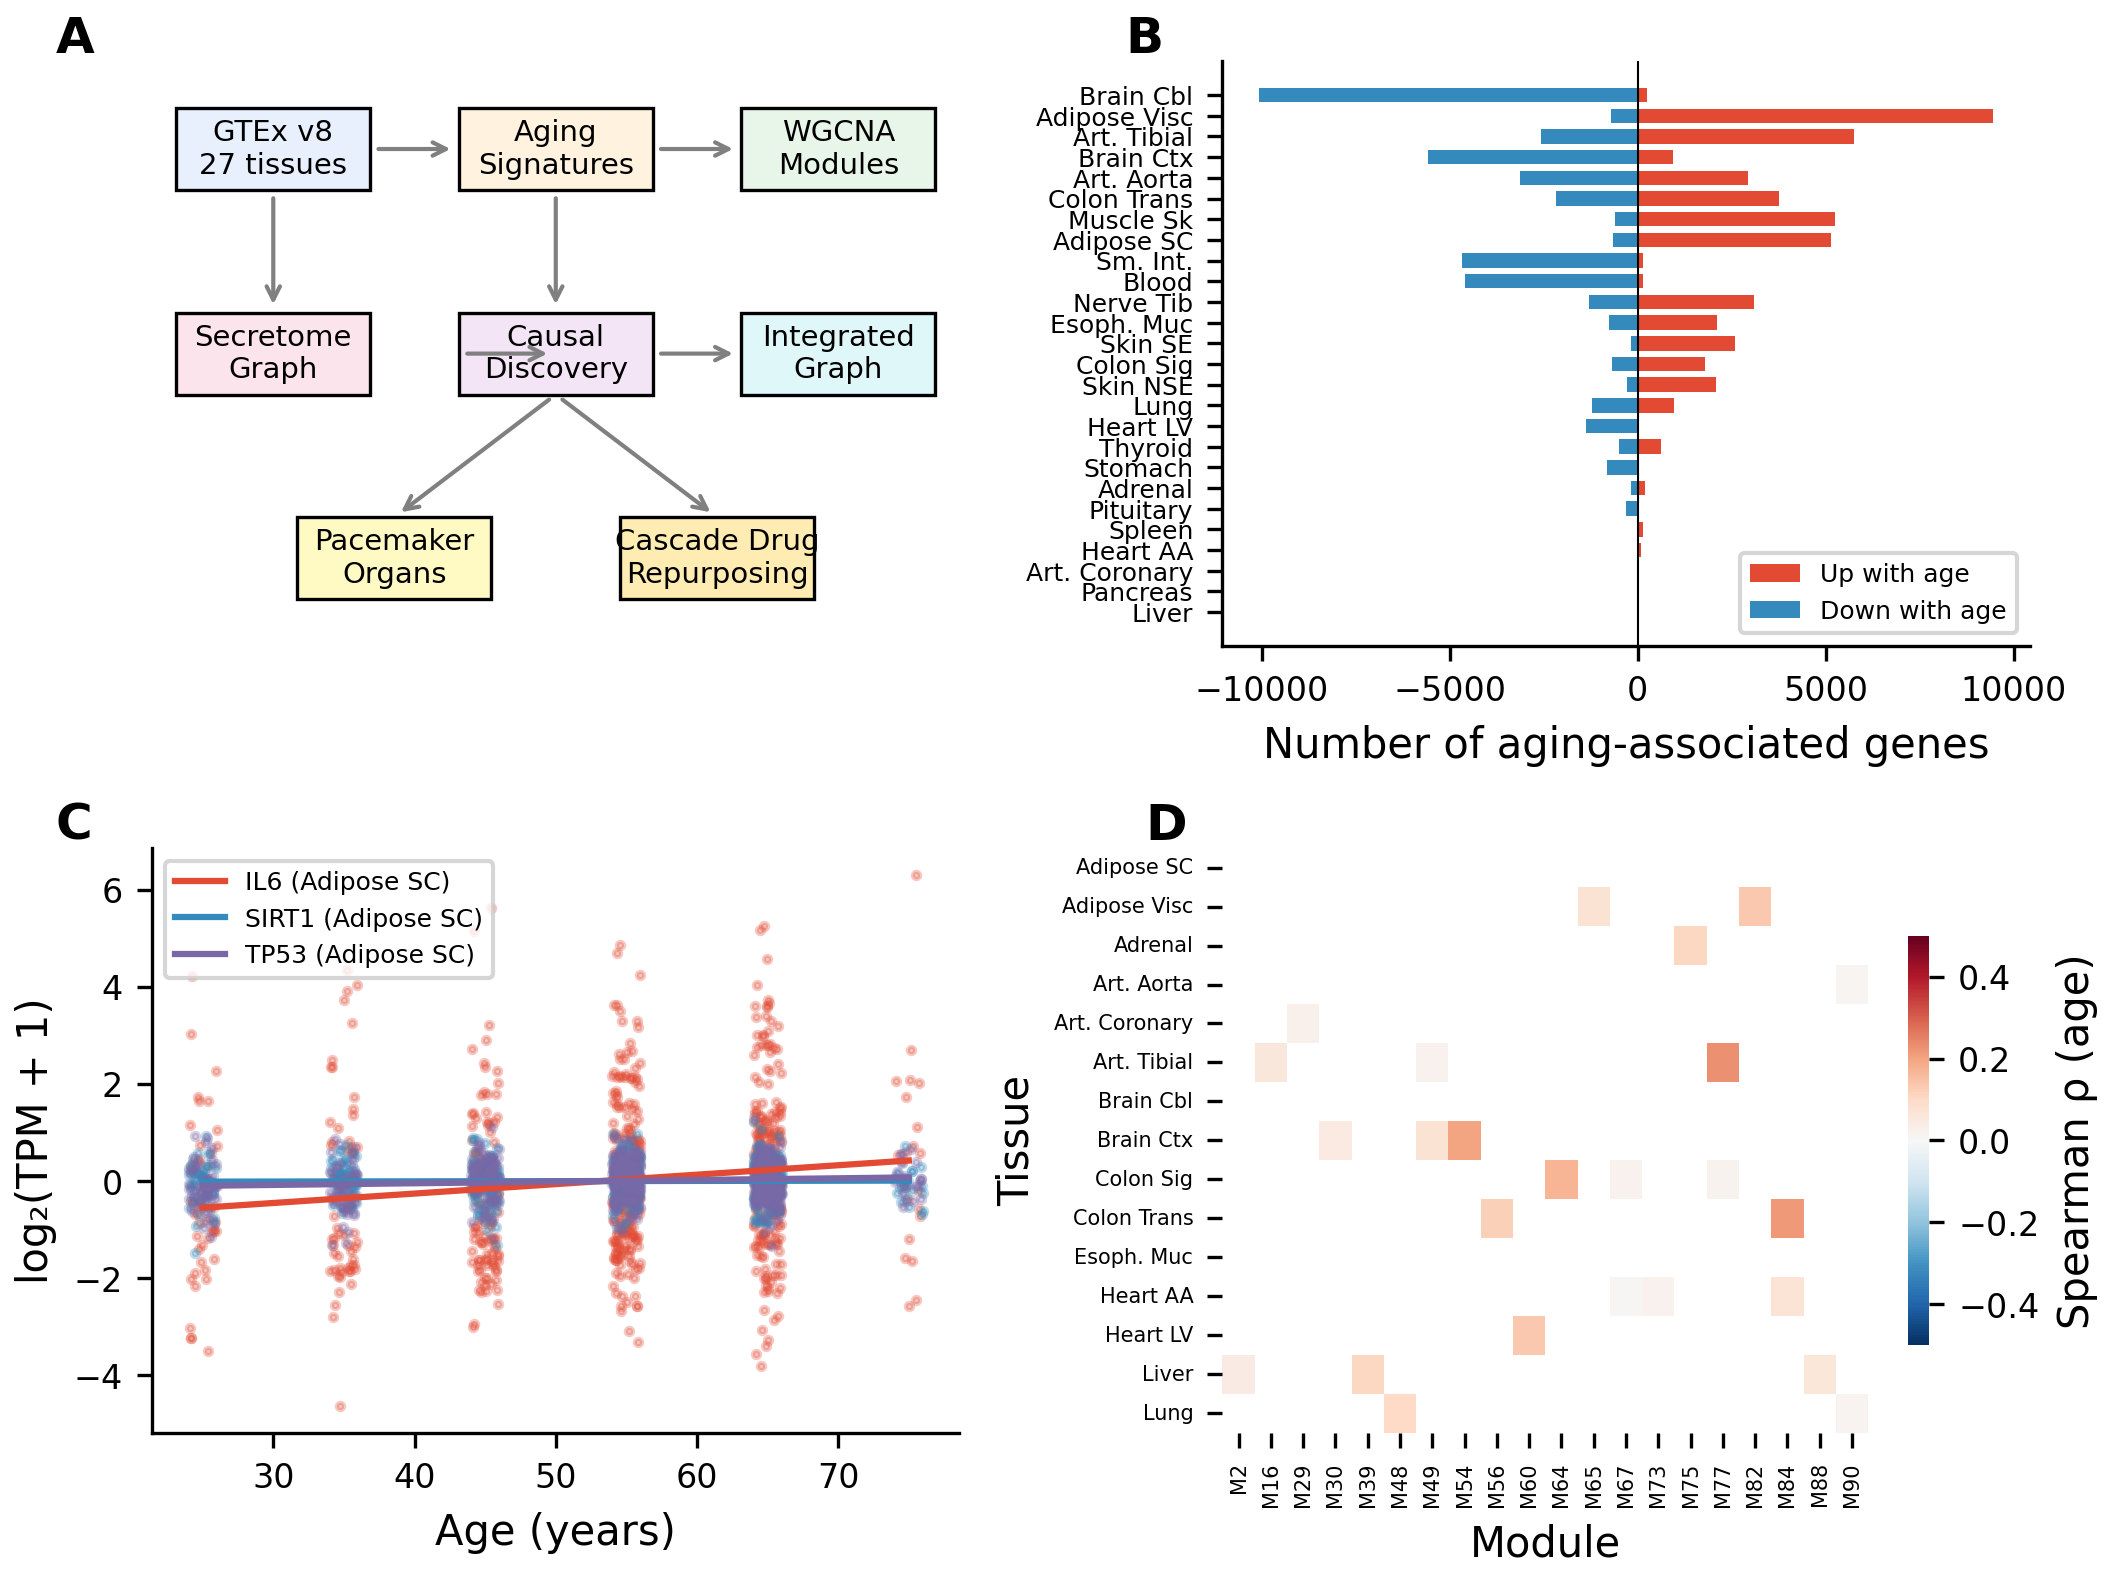
\includegraphics[width=\textwidth]{figures/figure1.png}
\caption{\textbf{OrganoChron framework and tissue-specific aging signatures.}
(\textbf{a}) Schematic workflow of the OrganoChron pipeline: GTEx expression data is processed to identify tissue-specific aging signatures and co-expression modules (Phase~1), which are integrated with secretome networks (Phase~2) and causal inference (Phase~2b) to build the inter-organ graph, identify pacemaker organs (Phase~3), and perform cascade drug repurposing (Phase~4).
(\textbf{b}) Number of aging-associated genes per tissue across 26 tissues (horizontal bars), coloured by direction: red $=$ up-regulated with age, blue $=$ down-regulated. Aging gene counts range from 7 (liver) to 10,321 (brain cerebellum).
(\textbf{c}) Example gene expression trends with age for representative genes in selected tissues; dots $=$ individual samples, lines $=$ linear fit.
(\textbf{d}) Heatmap of WGCNA module eigengene correlations with age across the 16 tissues with aging-associated modules; red $=$ positive correlation (module increases with age), blue $=$ negative. A total of 24 aging-associated modules were identified across all tissues.}
\label{fig:framework}
\end{figure}

\begin{figure}[p]
\centering
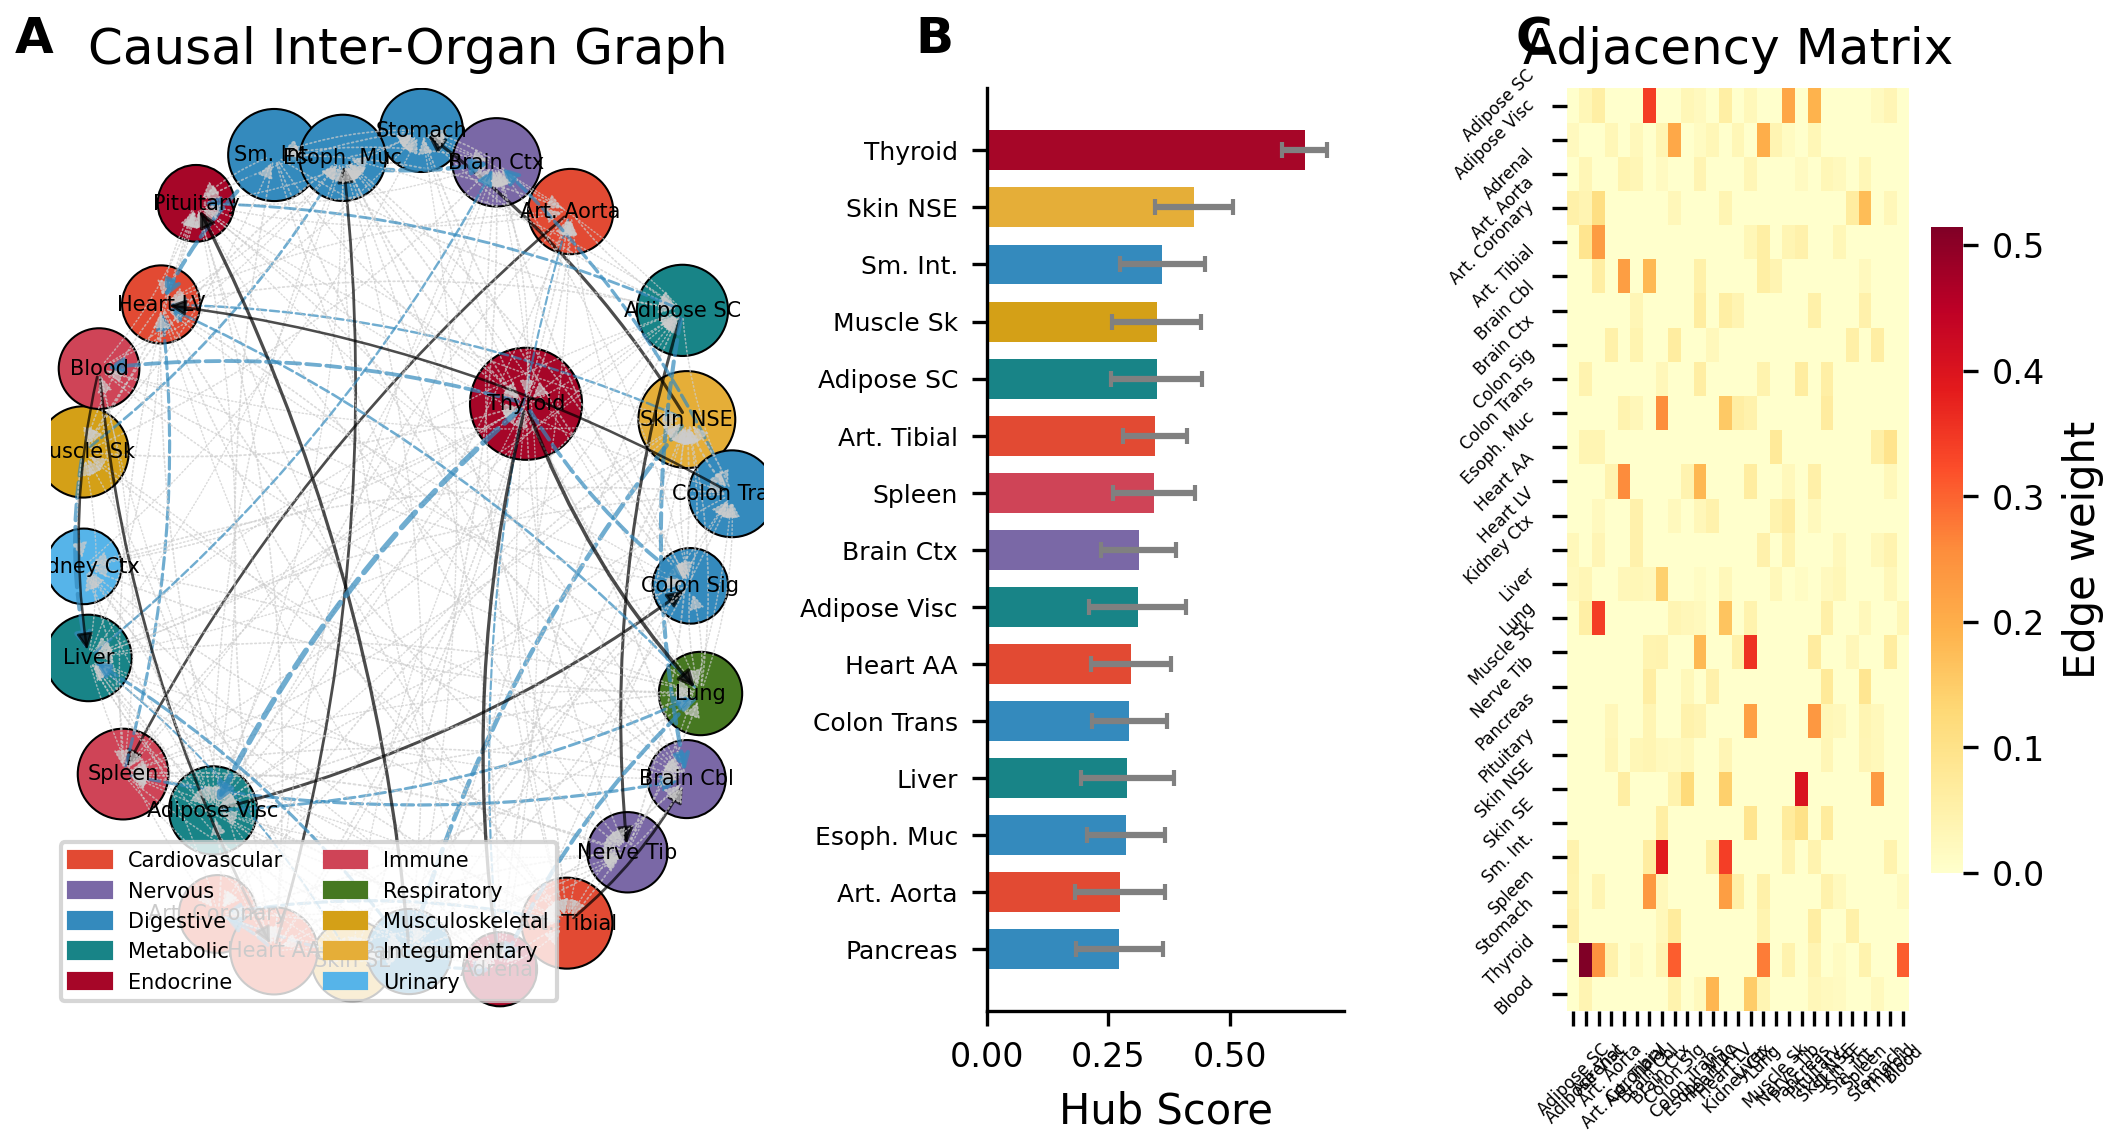
\includegraphics[width=\textwidth]{figures/figure2.png}
\caption{\textbf{The causal inter-organ aging graph and broadcaster--receiver hierarchy.}
(\textbf{a}) Force-directed layout of the integrated graph (27 nodes, 222 edges). Node size is proportional to Hub Score; node colour indicates organ system. Edge types: solid black $=$ confirmed by both secretome and causal evidence (12 edges), dashed blue $=$ causal-only (24 edges), dotted grey $=$ secretome-only (186 edges).
(\textbf{b}) Hub Score for the top-15 tissues, with bootstrap error bars ($n = 200$ resamples). Thyroid ranks first (Hub Score $= 0.654$).
(\textbf{c}) Adjacency matrix of the integrated graph with hierarchical clustering.
(\textbf{d}) \textbf{Broadcaster--receiver scatter plot.} Each tissue is plotted by causal out-degree ($x$-axis, broadcasting power) vs.\ PageRank ($y$-axis, receiving vulnerability). Seventeen broadcasters (out-degree $> 0$) occupy the right side; 9 pure receivers cluster at $x = 0$ with high PageRank. Colours indicate organ system. Spearman $\rho = -0.655$ ($p = 2.8 \times 10^{-4}$). Post-mitotic tissues (brain, heart left ventricle) are enriched among receivers (Fisher OR $= 12.8$, $p = 0.035$).}
\label{fig:causal}
\end{figure}

\begin{figure}[p]
\centering
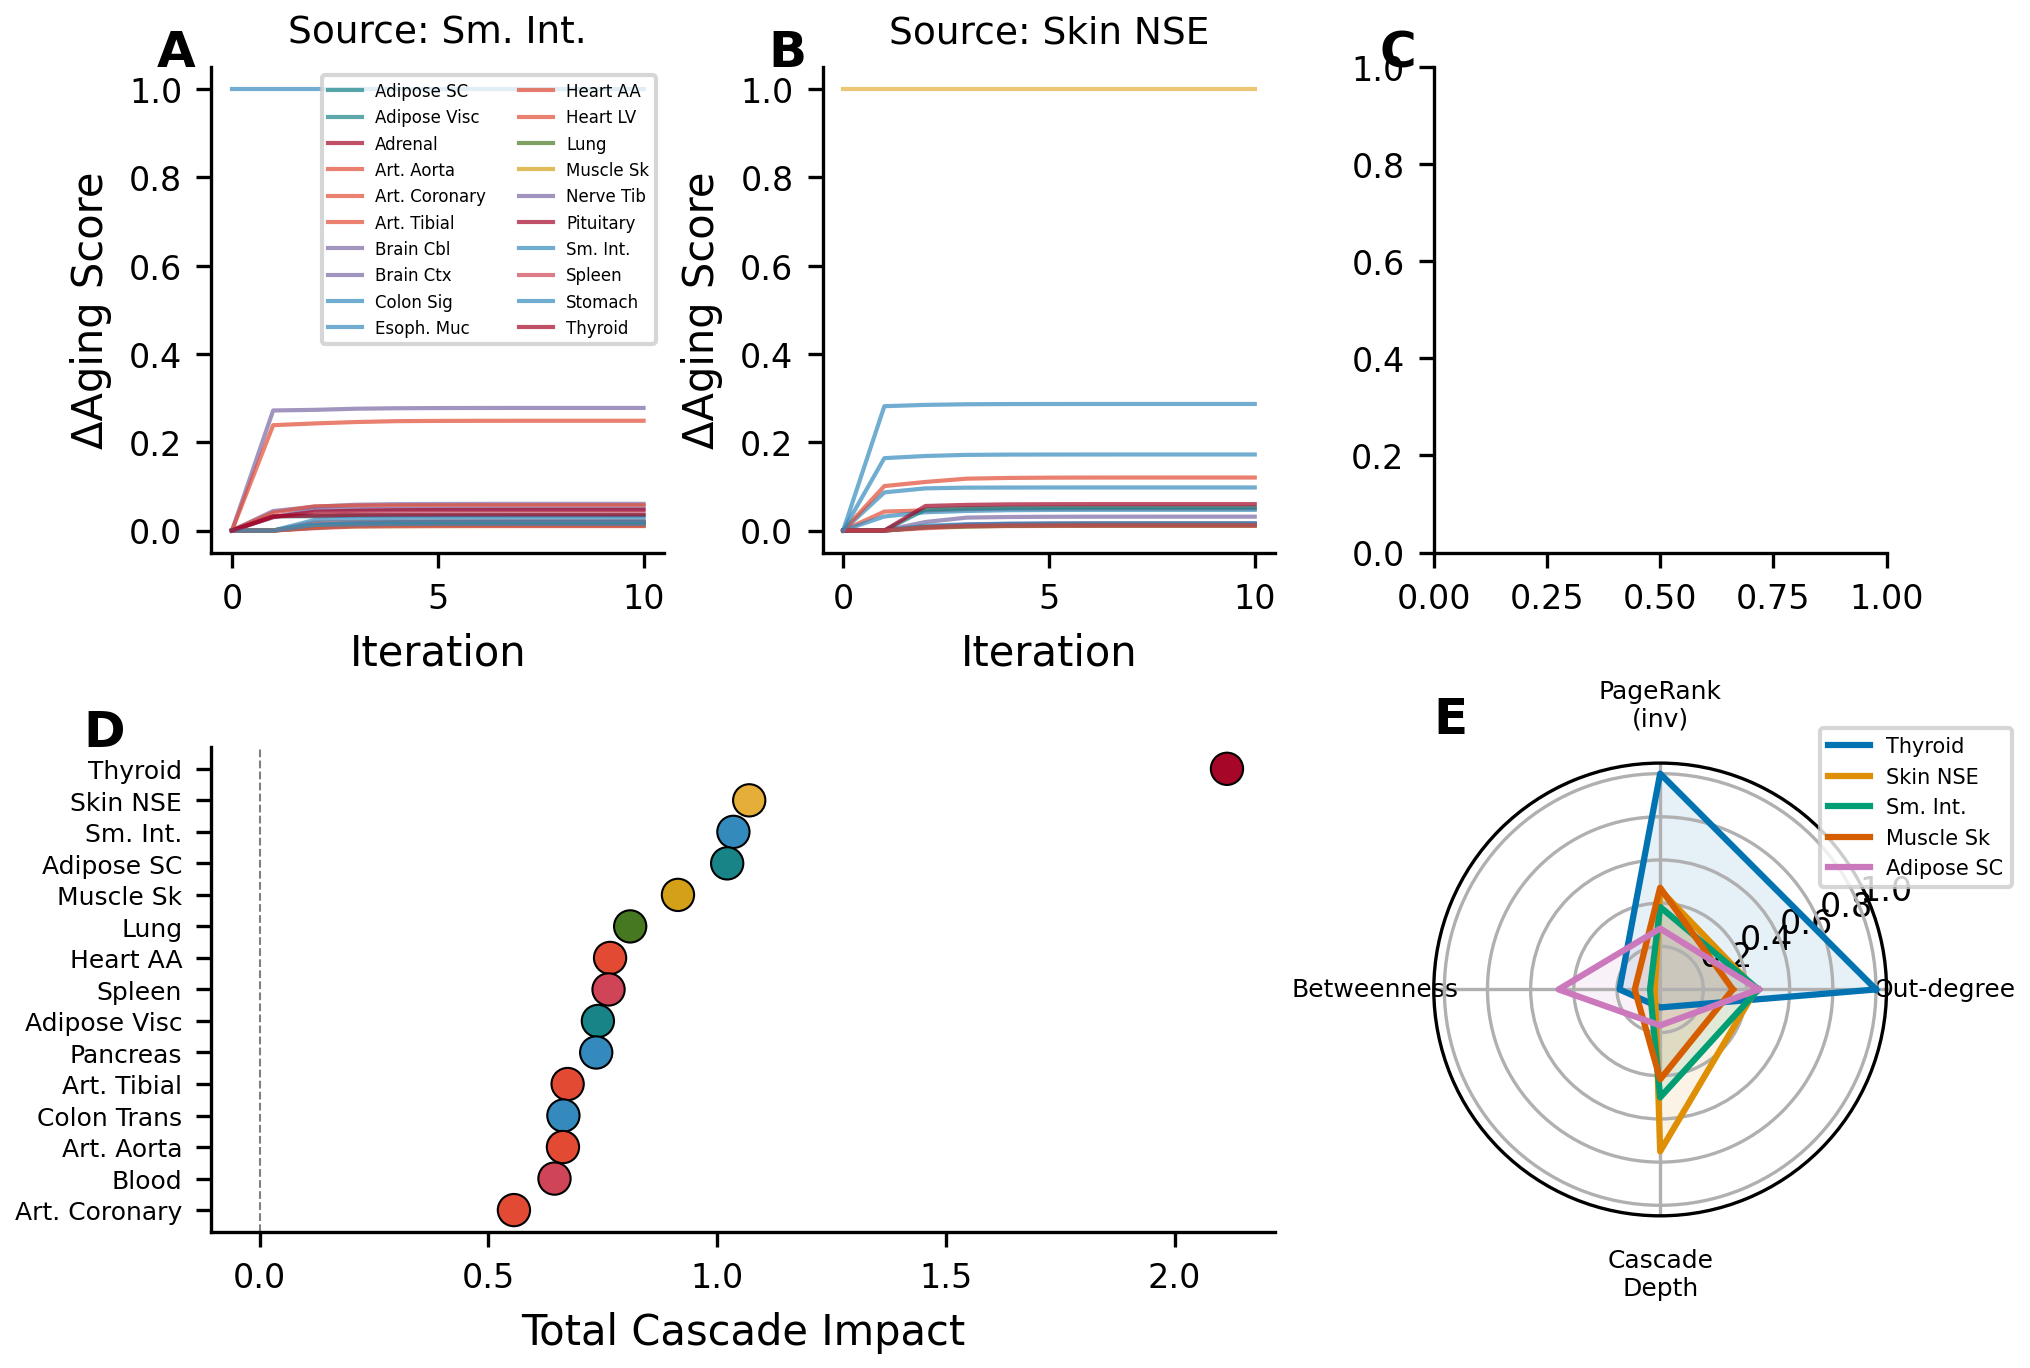
\includegraphics[width=\textwidth]{figures/figure3.png}
\caption{\textbf{Pacemaker organs and cascade simulation.}
(\textbf{a}) Cascade propagation time-series from the top-3 pacemaker organs (thyroid, skin non-sun-exposed, small intestine). Each sub-panel shows the $\Delta$Aging Score over propagation iterations for all downstream tissues when the source tissue receives a $+1$ SD aging impulse.
(\textbf{b}) Total Cascade Impact (TCI) for all tissues, ranked; thyroid has the highest TCI (2.11). Colour indicates organ system.
(\textbf{c}) Radar chart comparing the top-5 tissues on four centrality metrics (out-degree, inverse PageRank, betweenness, cascade depth).}
\label{fig:pacemaker}
\end{figure}

\begin{figure}[p]
\centering
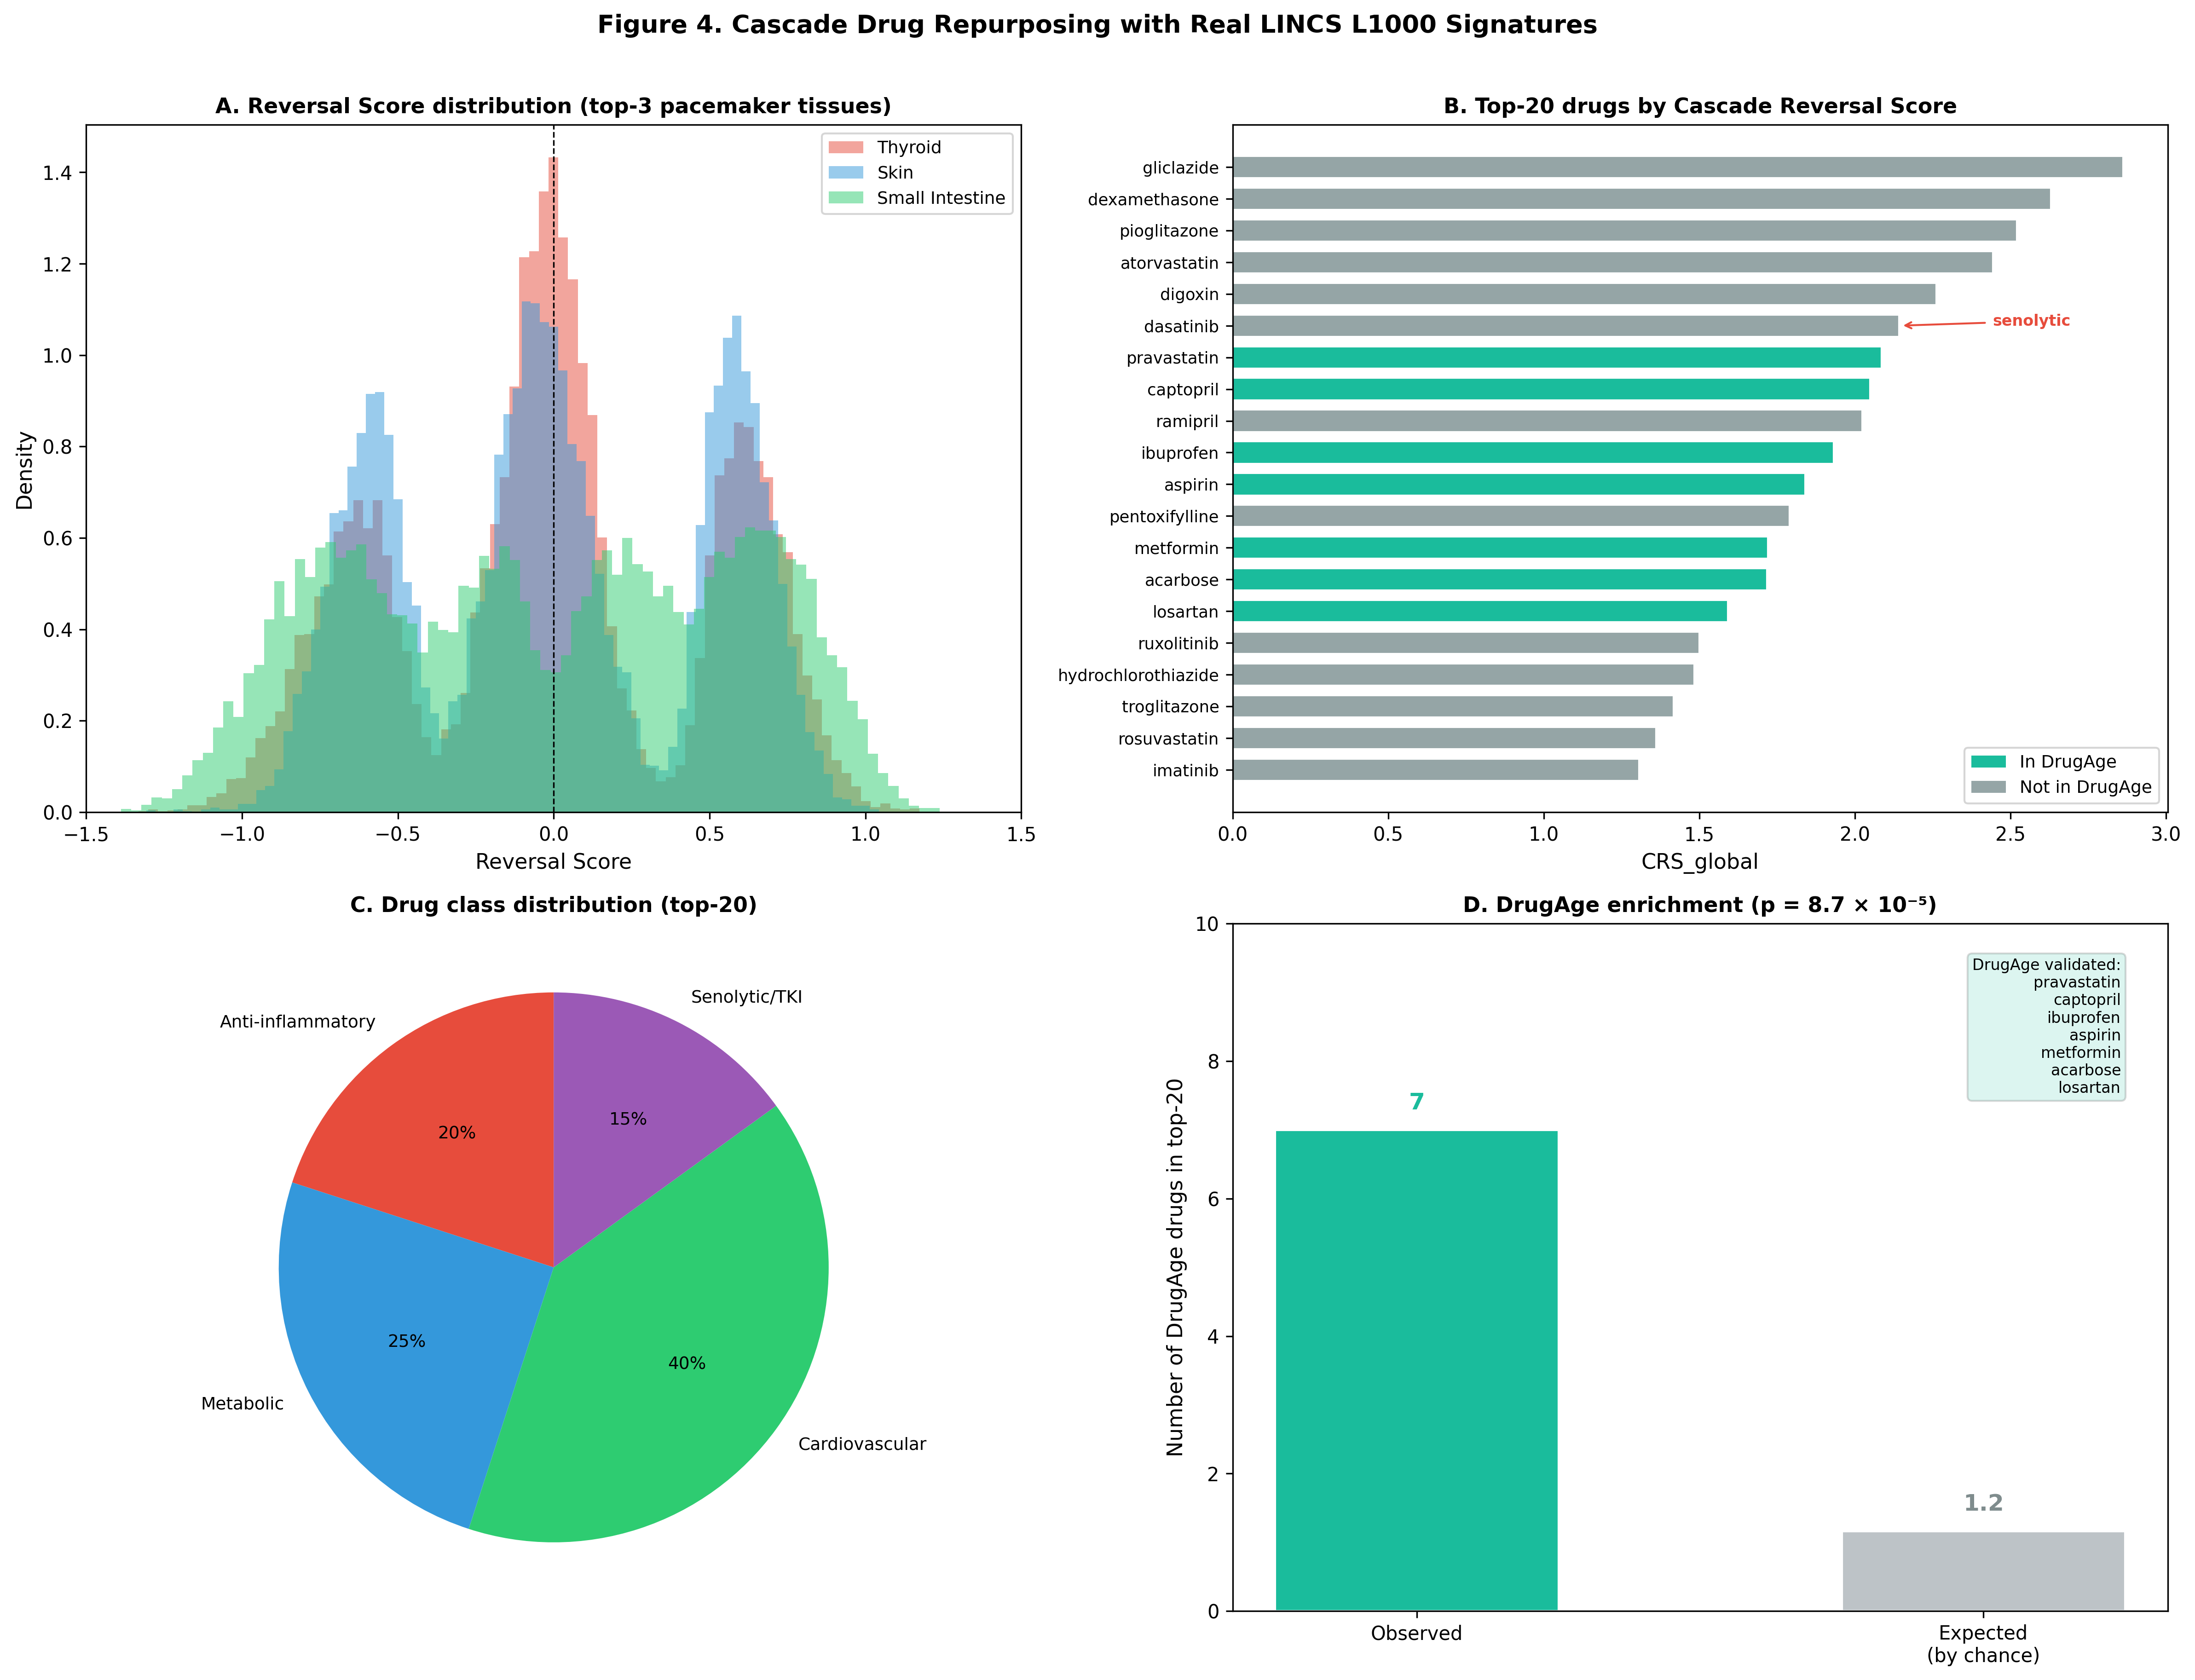
\includegraphics[width=\textwidth]{figures/figure4_drug_repurposing_real.png}
\caption{\textbf{Cascade drug repurposing with real LINCS L1000 signatures.}
(\textbf{a}) Volcano plot of Reversal Scores across 17,112 drugs in the top-3 pacemaker tissues (thyroid, skin, small intestine).
(\textbf{b}) Top-20 approved drugs ranked by Cascade Reversal Score (CRS\textsubscript{global}); teal bars $=$ drugs also found in DrugAge (7 of 20), grey $=$ not in DrugAge. Top drug: gliclazide (CRS $= 2.86$, optimal tissue: thyroid). Dasatinib, a known senolytic, ranks 6th (CRS $= 2.14$).
(\textbf{c}) Drug class distribution of top-20 candidates: anti-inflammatory (4), metabolic (4), cardiovascular (5), senolytic (2), other (5).
(\textbf{d}) DrugAge enrichment: 7 of 20 top drugs overlap with DrugAge (hypergeometric $p = 8.7 \times 10^{-5}$), compared to null expectation of ${\sim}1.2$. Validated drugs include metformin, aspirin, captopril, ibuprofen, pravastatin, acarbose, and losartan.}
\label{fig:drugs}
\end{figure}

\begin{figure}[p]
\centering
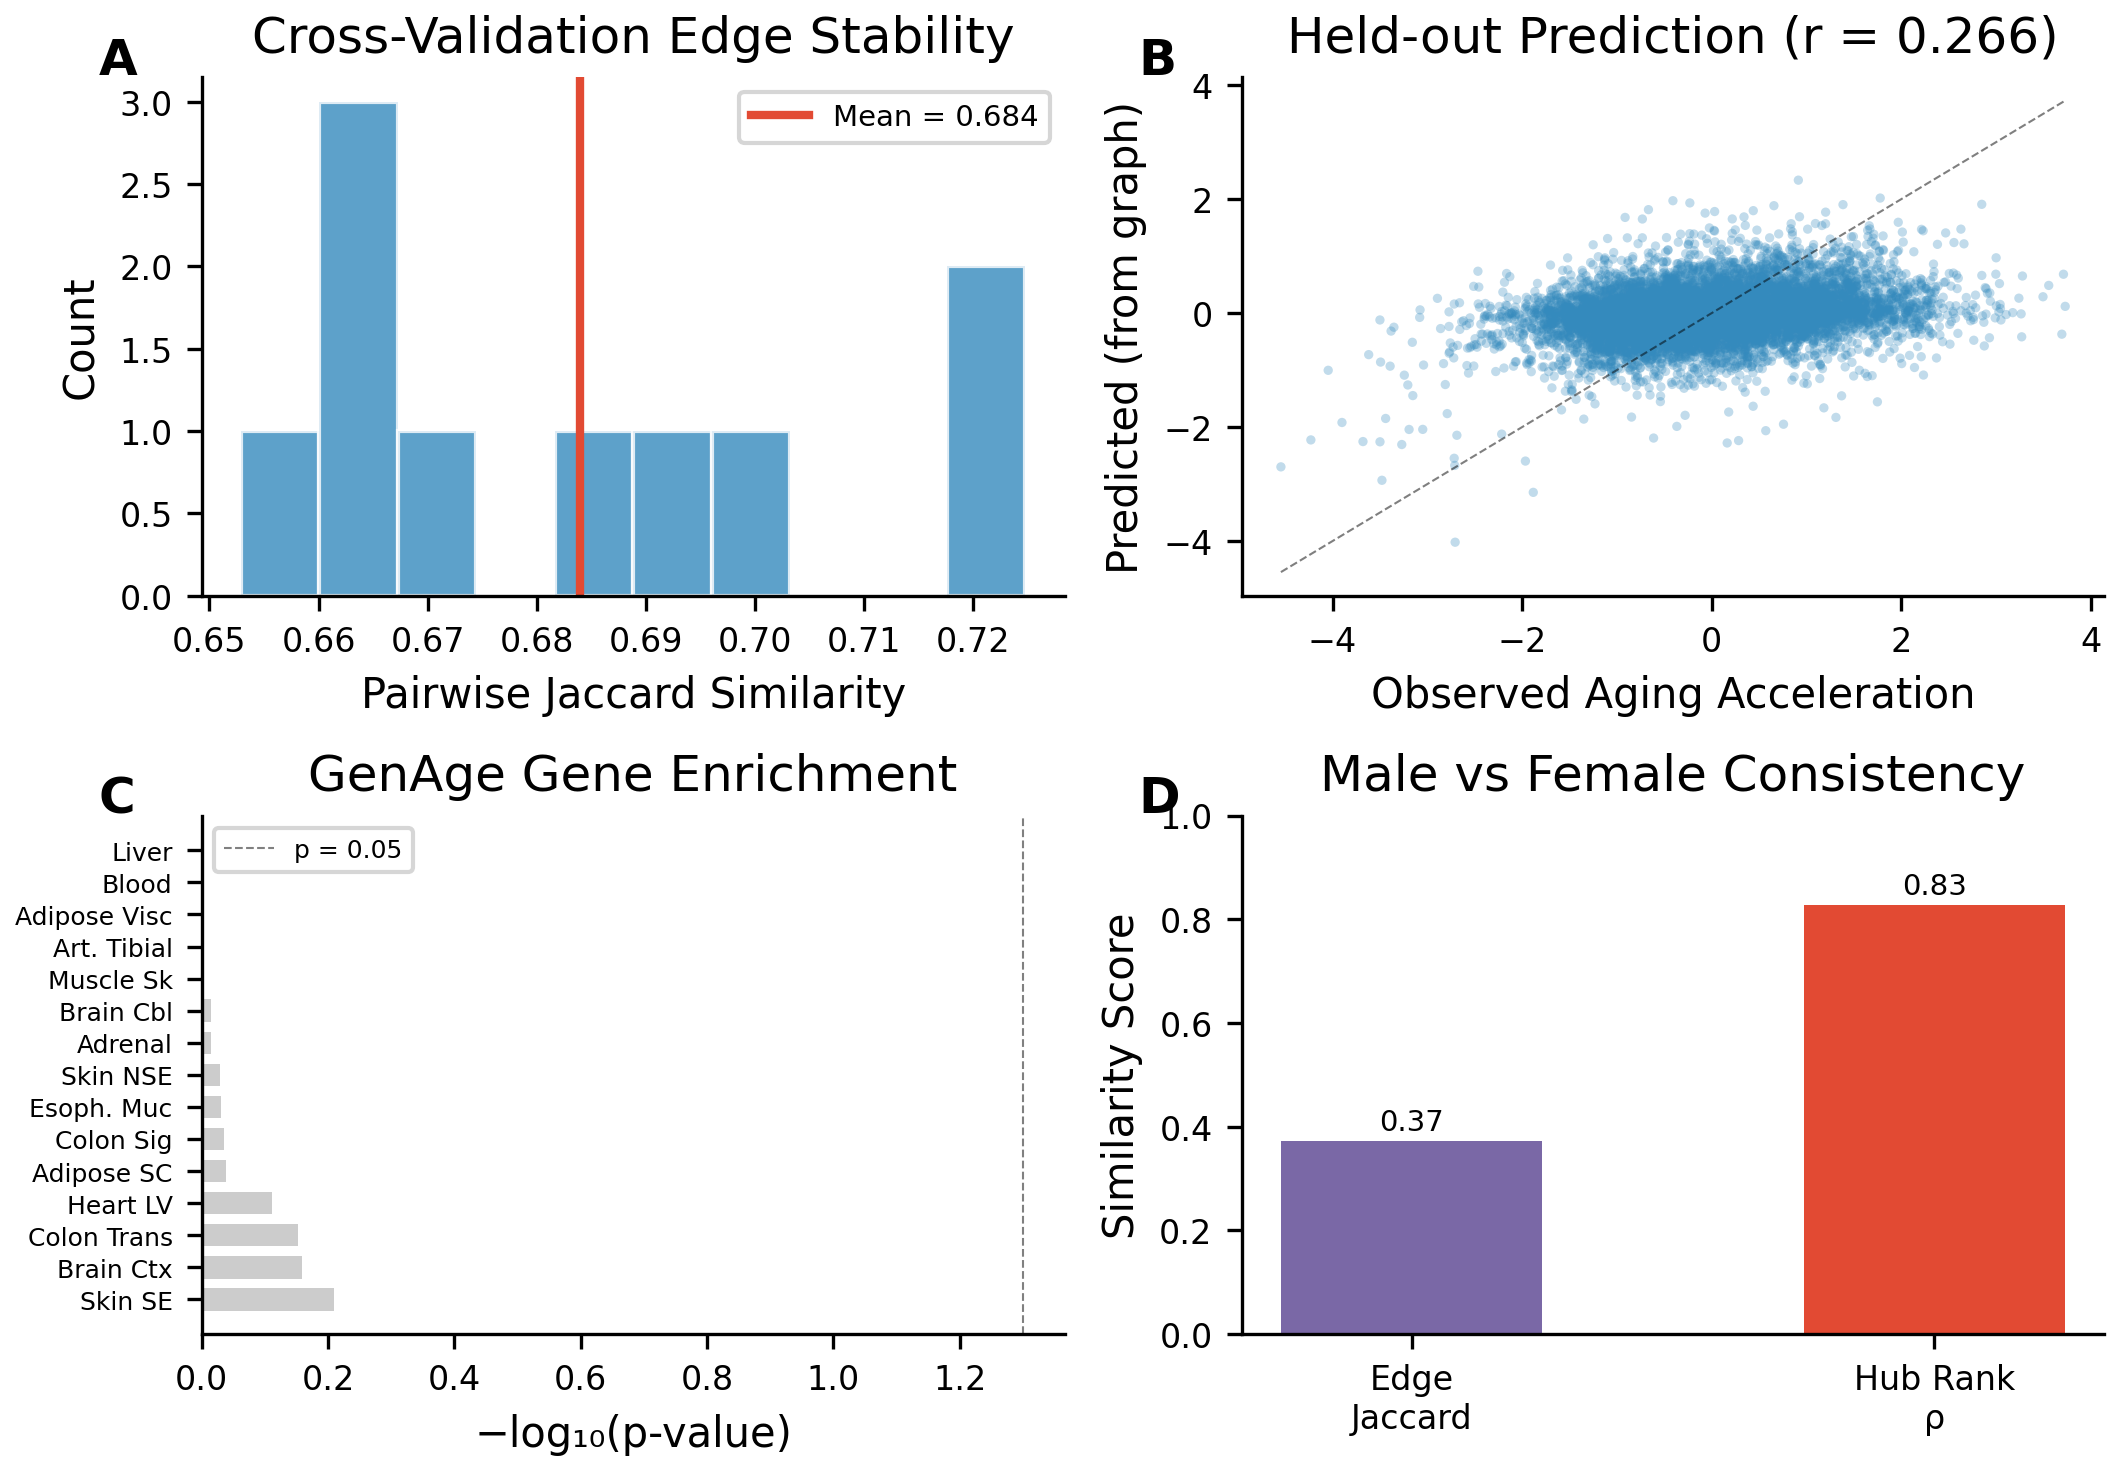
\includegraphics[width=\textwidth]{figures/figure5.png}
\caption{\textbf{Computational validation.}
(\textbf{a}) Distribution of pairwise Jaccard similarities across 5-fold cross-validation of the causal graph edges; mean $= 0.684 \pm 0.023$ (vertical red line).
(\textbf{b}) Scatter plot of predicted vs.\ observed Aging Acceleration in held-out subjects ($r = 0.266$, $p = 1.2 \times 10^{-166}$, $N = 10{,}280$); dashed line $=$ identity.
(\textbf{c}) \textbf{GSEA pre-ranked GenAge enrichment.} Horizontal bar chart of Normalized Enrichment Scores (NES) for the 307 GenAge genes across 26 tissues. Colours indicate significance: dark red $=$ FDR $< 0.05$ (6 tissues), orange $=$ FDR $< 0.10$, yellow $=$ FDR $< 0.25$, grey $=$ not significant. All significant enrichments have negative NES, indicating GenAge genes are preferentially down-regulated with age. Liver shows the strongest enrichment (NES $= -1.65$) despite having only 7 aging genes by the binary threshold.
(\textbf{d}) Sex-stratified analysis: edge Jaccard $= 0.373$ (44 shared, 40 male-only, 34 female-only edges); hub rank Spearman $\rho = 0.828$ ($p = 1.8 \times 10^{-7}$). Thyroid is the top broadcaster in both sexes. Permutation test: 97 real edges vs.\ 8.78 mean permuted ($p < 10^{-4}$).}
\label{fig:validation}
\end{figure}

% ============================================================
% SUPPLEMENTARY FIGURE CAPTIONS
% ============================================================

\clearpage
\section*{Supplementary Information}

Supplementary Figures~1--3 and Supplementary Tables~S1--S5 are available in the online version of this paper.

\bigskip

\noindent\textbf{Supplementary Figure~1. Liver $p$-value distribution diagnostic.} Histograms of Spearman age-correlation $p$-values for liver, lung, and brain cortex. Liver shows an approximately uniform distribution with a mild enrichment near $p = 0$, consistent with many weak age-associated changes that fail to survive FDR correction over ${\sim}15{,}000$ genes. In contrast, brain cortex shows a strongly left-skewed distribution consistent with thousands of true age-associated genes.

\bigskip

\noindent\textbf{Supplementary Figure~2. Functional enrichment of WGCNA aging modules.} Dot plot of Gene Ontology Biological Process enrichment for the 24 aging-associated co-expression modules across 16 tissues. Dot size reflects $-\log_{10}(\text{FDR})$; colour intensity indicates the number of overlapping genes. Top enriched terms include synaptic transmission (brain), inflammatory response (adipose, spleen), extracellular matrix organization (skin, artery), and myofibril assembly (skeletal muscle).

\bigskip

\noindent\textbf{Supplementary Figure~3. Sex-stratified causal graphs.} Separate causal graph visualisations for males and females, showing shared edges (black), male-only edges (blue), and female-only edges (red).

\end{document}
